% Options for packages loaded elsewhere
\PassOptionsToPackage{unicode}{hyperref}
\PassOptionsToPackage{hyphens}{url}
%
\documentclass[
  10pt,
]{article}
\usepackage{amsmath,amssymb}
\usepackage{iftex}
\ifPDFTeX
  \usepackage[T1]{fontenc}
  \usepackage[utf8]{inputenc}
  \usepackage{textcomp} % provide euro and other symbols
\else % if luatex or xetex
  \usepackage{unicode-math} % this also loads fontspec
  \defaultfontfeatures{Scale=MatchLowercase}
  \defaultfontfeatures[\rmfamily]{Ligatures=TeX,Scale=1}
\fi
\usepackage{lmodern}
\ifPDFTeX\else
  % xetex/luatex font selection
\fi
% Use upquote if available, for straight quotes in verbatim environments
\IfFileExists{upquote.sty}{\usepackage{upquote}}{}
\IfFileExists{microtype.sty}{% use microtype if available
  \usepackage[]{microtype}
  \UseMicrotypeSet[protrusion]{basicmath} % disable protrusion for tt fonts
}{}
\makeatletter
\@ifundefined{KOMAClassName}{% if non-KOMA class
  \IfFileExists{parskip.sty}{%
    \usepackage{parskip}
  }{% else
    \setlength{\parindent}{0pt}
    \setlength{\parskip}{6pt plus 2pt minus 1pt}}
}{% if KOMA class
  \KOMAoptions{parskip=half}}
\makeatother
\usepackage{xcolor}
\usepackage[margin=1in]{geometry}
\usepackage{color}
\usepackage{fancyvrb}
\newcommand{\VerbBar}{|}
\newcommand{\VERB}{\Verb[commandchars=\\\{\}]}
\DefineVerbatimEnvironment{Highlighting}{Verbatim}{commandchars=\\\{\}}
% Add ',fontsize=\small' for more characters per line
\usepackage{framed}
\definecolor{shadecolor}{RGB}{248,248,248}
\newenvironment{Shaded}{\begin{snugshade}}{\end{snugshade}}
\newcommand{\AlertTok}[1]{\textcolor[rgb]{0.94,0.16,0.16}{#1}}
\newcommand{\AnnotationTok}[1]{\textcolor[rgb]{0.56,0.35,0.01}{\textbf{\textit{#1}}}}
\newcommand{\AttributeTok}[1]{\textcolor[rgb]{0.13,0.29,0.53}{#1}}
\newcommand{\BaseNTok}[1]{\textcolor[rgb]{0.00,0.00,0.81}{#1}}
\newcommand{\BuiltInTok}[1]{#1}
\newcommand{\CharTok}[1]{\textcolor[rgb]{0.31,0.60,0.02}{#1}}
\newcommand{\CommentTok}[1]{\textcolor[rgb]{0.56,0.35,0.01}{\textit{#1}}}
\newcommand{\CommentVarTok}[1]{\textcolor[rgb]{0.56,0.35,0.01}{\textbf{\textit{#1}}}}
\newcommand{\ConstantTok}[1]{\textcolor[rgb]{0.56,0.35,0.01}{#1}}
\newcommand{\ControlFlowTok}[1]{\textcolor[rgb]{0.13,0.29,0.53}{\textbf{#1}}}
\newcommand{\DataTypeTok}[1]{\textcolor[rgb]{0.13,0.29,0.53}{#1}}
\newcommand{\DecValTok}[1]{\textcolor[rgb]{0.00,0.00,0.81}{#1}}
\newcommand{\DocumentationTok}[1]{\textcolor[rgb]{0.56,0.35,0.01}{\textbf{\textit{#1}}}}
\newcommand{\ErrorTok}[1]{\textcolor[rgb]{0.64,0.00,0.00}{\textbf{#1}}}
\newcommand{\ExtensionTok}[1]{#1}
\newcommand{\FloatTok}[1]{\textcolor[rgb]{0.00,0.00,0.81}{#1}}
\newcommand{\FunctionTok}[1]{\textcolor[rgb]{0.13,0.29,0.53}{\textbf{#1}}}
\newcommand{\ImportTok}[1]{#1}
\newcommand{\InformationTok}[1]{\textcolor[rgb]{0.56,0.35,0.01}{\textbf{\textit{#1}}}}
\newcommand{\KeywordTok}[1]{\textcolor[rgb]{0.13,0.29,0.53}{\textbf{#1}}}
\newcommand{\NormalTok}[1]{#1}
\newcommand{\OperatorTok}[1]{\textcolor[rgb]{0.81,0.36,0.00}{\textbf{#1}}}
\newcommand{\OtherTok}[1]{\textcolor[rgb]{0.56,0.35,0.01}{#1}}
\newcommand{\PreprocessorTok}[1]{\textcolor[rgb]{0.56,0.35,0.01}{\textit{#1}}}
\newcommand{\RegionMarkerTok}[1]{#1}
\newcommand{\SpecialCharTok}[1]{\textcolor[rgb]{0.81,0.36,0.00}{\textbf{#1}}}
\newcommand{\SpecialStringTok}[1]{\textcolor[rgb]{0.31,0.60,0.02}{#1}}
\newcommand{\StringTok}[1]{\textcolor[rgb]{0.31,0.60,0.02}{#1}}
\newcommand{\VariableTok}[1]{\textcolor[rgb]{0.00,0.00,0.00}{#1}}
\newcommand{\VerbatimStringTok}[1]{\textcolor[rgb]{0.31,0.60,0.02}{#1}}
\newcommand{\WarningTok}[1]{\textcolor[rgb]{0.56,0.35,0.01}{\textbf{\textit{#1}}}}
\usepackage{longtable,booktabs,array}
\usepackage{calc} % for calculating minipage widths
% Correct order of tables after \paragraph or \subparagraph
\usepackage{etoolbox}
\makeatletter
\patchcmd\longtable{\par}{\if@noskipsec\mbox{}\fi\par}{}{}
\makeatother
% Allow footnotes in longtable head/foot
\IfFileExists{footnotehyper.sty}{\usepackage{footnotehyper}}{\usepackage{footnote}}
\makesavenoteenv{longtable}
\usepackage{graphicx}
\makeatletter
\def\maxwidth{\ifdim\Gin@nat@width>\linewidth\linewidth\else\Gin@nat@width\fi}
\def\maxheight{\ifdim\Gin@nat@height>\textheight\textheight\else\Gin@nat@height\fi}
\makeatother
% Scale images if necessary, so that they will not overflow the page
% margins by default, and it is still possible to overwrite the defaults
% using explicit options in \includegraphics[width, height, ...]{}
\setkeys{Gin}{width=\maxwidth,height=\maxheight,keepaspectratio}
% Set default figure placement to htbp
\makeatletter
\def\fps@figure{htbp}
\makeatother
\setlength{\emergencystretch}{3em} % prevent overfull lines
\providecommand{\tightlist}{%
  \setlength{\itemsep}{0pt}\setlength{\parskip}{0pt}}
\setcounter{secnumdepth}{-\maxdimen} % remove section numbering
\usepackage{graphicx}
\usepackage{geometry}
\geometry{margin=1in}
\usepackage{tocbibind}
\usepackage{titlesec}
\usepackage{titling}
\usepackage{fancyhdr}
\pagestyle{fancy}
\fancyhf{}
\fancyhead[L]{
\includegraphics[width=0.1\textwidth]{img_rmd/logo1.jpg}}
\fancyhead[R]{
\includegraphics[width=0.1\textwidth]{img_rmd/logo2.jpg}}
\renewcommand{\headrulewidth}{1pt}
\fancyfoot[C]{\thepage}
\fancyhead[C]{\nouppercase{\leftmark}}
\renewcommand{\headrulewidth}{0.4pt}
\pretitle{\begin{center}
\includegraphics[width=0.3\textwidth]{img_rmd/logo1.jpg}\hfill
\includegraphics[width=0.3\textwidth]{img_rmd/logo2.jpg}\vskip 2em\LARGE}
\posttitle{\end{center}\vskip 1.5em}
\preauthor{\begin{center}\Large\lineskip 0.5em}
\postauthor{\par\end{center}}
\predate{\begin{center}\large}
\postdate{\par\end{center}\vfill}
\ifLuaTeX
  \usepackage{selnolig}  % disable illegal ligatures
\fi
\usepackage{bookmark}
\IfFileExists{xurl.sty}{\usepackage{xurl}}{} % add URL line breaks if available
\urlstyle{same}
\hypersetup{
  pdftitle={Rapport de Stage L3},
  pdfauthor={Gilibert Rémy},
  hidelinks,
  pdfcreator={LaTeX via pandoc}}

\title{Rapport de Stage L3}
\author{Gilibert Rémy}
\date{06/05/2024 au 07/07/2024}

\begin{document}
\maketitle

\newpage

\thispagestyle{empty}
\begin{center}
  \Huge{\textbf{Table des Matières}}
\end{center}
\tableofcontents
\newpage

\section{Remerciements}\label{remerciements}

Je tiens à remercier :

Jérôme Pasquet pour cette opportunité de stage ainsi que pour les
connaissances acquises durant le semestre 5 grâce a sont cours de
développement web.

Théo Oriol pour m'avoir suivie tout au long de ce stage en corrigeant
mes erreurs et m'orientant vers la bonne direction

Pierre Jay-Robert et toute l'équipe du CEFE de m'avoir accueillie au
sein de leur structure et en particulier Ninon Delcourt qui a accepté de
partager son bureau avec moi tout au long de mon stage.

Daniel Gilibert /languageTool/Chatgpt pour la correction orthographique
de ce rapport.

Maximilien servajean pour le cours de programmation orienter objet qui
m'ont permis d'avoir les bases de python.

\newpage

\section{Introduction}\label{introduction}

Actuellement étudiant en 3ème année de MIASHS (mathématique et
informatique appliqué aux sciences humaines et sociales) à l'université
Paul Valéry Montpellier 3, j'ai eu la chance d'effectuer mon stage de
fin de licence du 06/05/2024 au 07/05/2024 au sein du Centre d'écologie
fonctionnelle et évolutive (sections du CEFE situé au campus Paul
Valery) où j'ai pu découvrir le travail dans un laboratoire de
recherche.

\begin{quote}
« Le CEFE est un des plus importants laboratoires de recherche en
Ecologie en France. Le projet du CEFE vise à comprendre la dynamique, le
fonctionnement et l'évolution du vivant de «la bactérie à l'éléphant »
et « du génome à la planète ». Il s'appuie sur trois ambitions: {[}1{]}
comprendre le monde vivant pour anticiper ce que sera demain {[}2{]}
conduire à des innovations et répondre aux attentes de la société;
{[}3{]} pratiquer une science « rassembleuse » et diverse dans ses
approches disciplinaires. Les questions de recherche sont posées dans un
contexte marqué par la prégnance des changements planétaires, le
développement de nouvelles technologies de manipulation du vivant et
l'exigence croissante de la société pour la recherche. »
\end{quote}

Source: \href{https://www.cefe.cnrs.fr/fr/}{CEFE}

Durant ce stage, j'ai pu créer en collaboration avec Théo Oriol
(Doctorant) une interface web dédiée à l'identification des collemboles
grâce à la reconnaissance sur image (YOLO v5x6) ainsi qu'à
l'amélioration du modèle via un système d'annotation. Ce sujet de stage
m'a permis de manipuler plusieurs outils pour le développement web comme
Flask et Bootstrap mais aussi plusieurs concepts du Deep Learning comme
l'implémentation d'un modèle ``l'Active Learning'' lié à ce dernier
ainsi que le ``Fine Tuning''. Cette interface web permettra à termes aux
chercheurs et passionnés du monde entier d'avoir accès à une
identification rapide et fiable, évitant les pertes de temps liées à
cette partie, et permettra d'améliorer continuellement le modèle tout en
collectant les données fournies par les utilisateurs de l'interface.

\newpage

\section{Présentation du travail
réalisé}\label{pruxe9sentation-du-travail-ruxe9alisuxe9}

\subsection{Développement web}\label{duxe9veloppement-web}

\subsubsection{Inscription / connexion}\label{inscription-connexion}

Les premières choses réalisées sur l'interface web furent la mise en
place des pages d'inscription et de connexion ainsi que la création
d'une base de données. La mise en place de ces pages nécessita
premièrement des recherches poussées et précises sur le framework
``Flask'' pour apprendre à créer des pages web via des applications
ainsi que les syntaxes et méthodes spécifiques à Flask. Une première
interface web a donc été créée pour les pages inscription et connexion
(Fig 1 et 2). La création de la base de données a été faite à la même
période permettant le stockage des informations utiles comme le nom
d'utilisateur, le mot de passe (haché au préalable) et pour finir, on
stocke aussi à l'inscription le paramètre ``expert'' ou non expert pour
des questions d'accessibilité que nous traiterons plus tard. Dans cette
même semaine, une Nav-bar a été ajoutée, elle contiendra tous les liens
utiles vers les autres pages du site web et permettra aussi la
déconnexion qui remplace connexion et inscription si vous êtes connecté.

\begin{figure}[htbp]
\centering
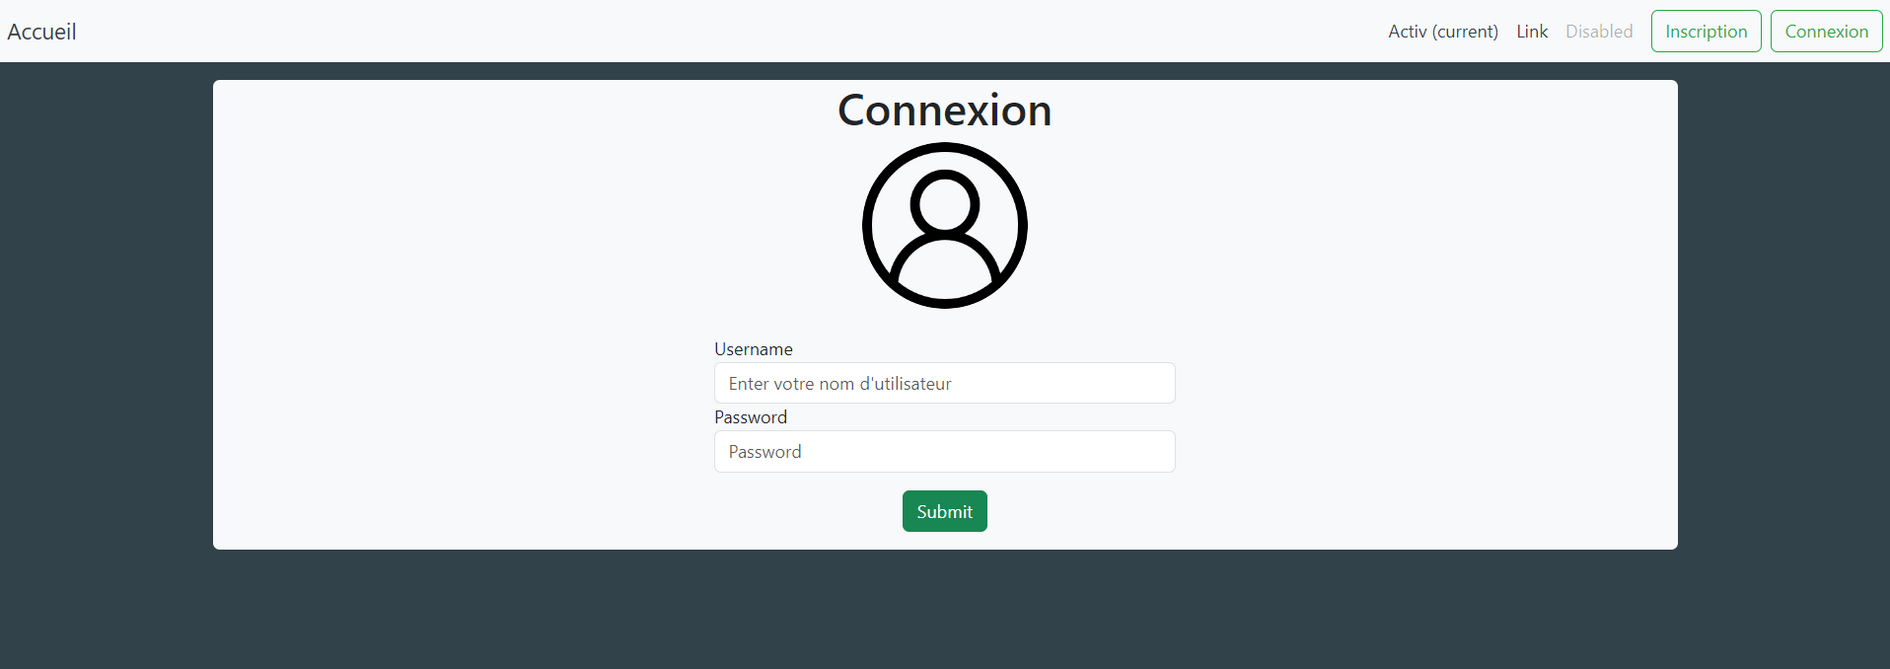
\includegraphics[width=\textwidth]{img_rmd/fig1.png}
\caption{Page d'inscription}
\end{figure}

\begin{figure}[htbp]
\centering
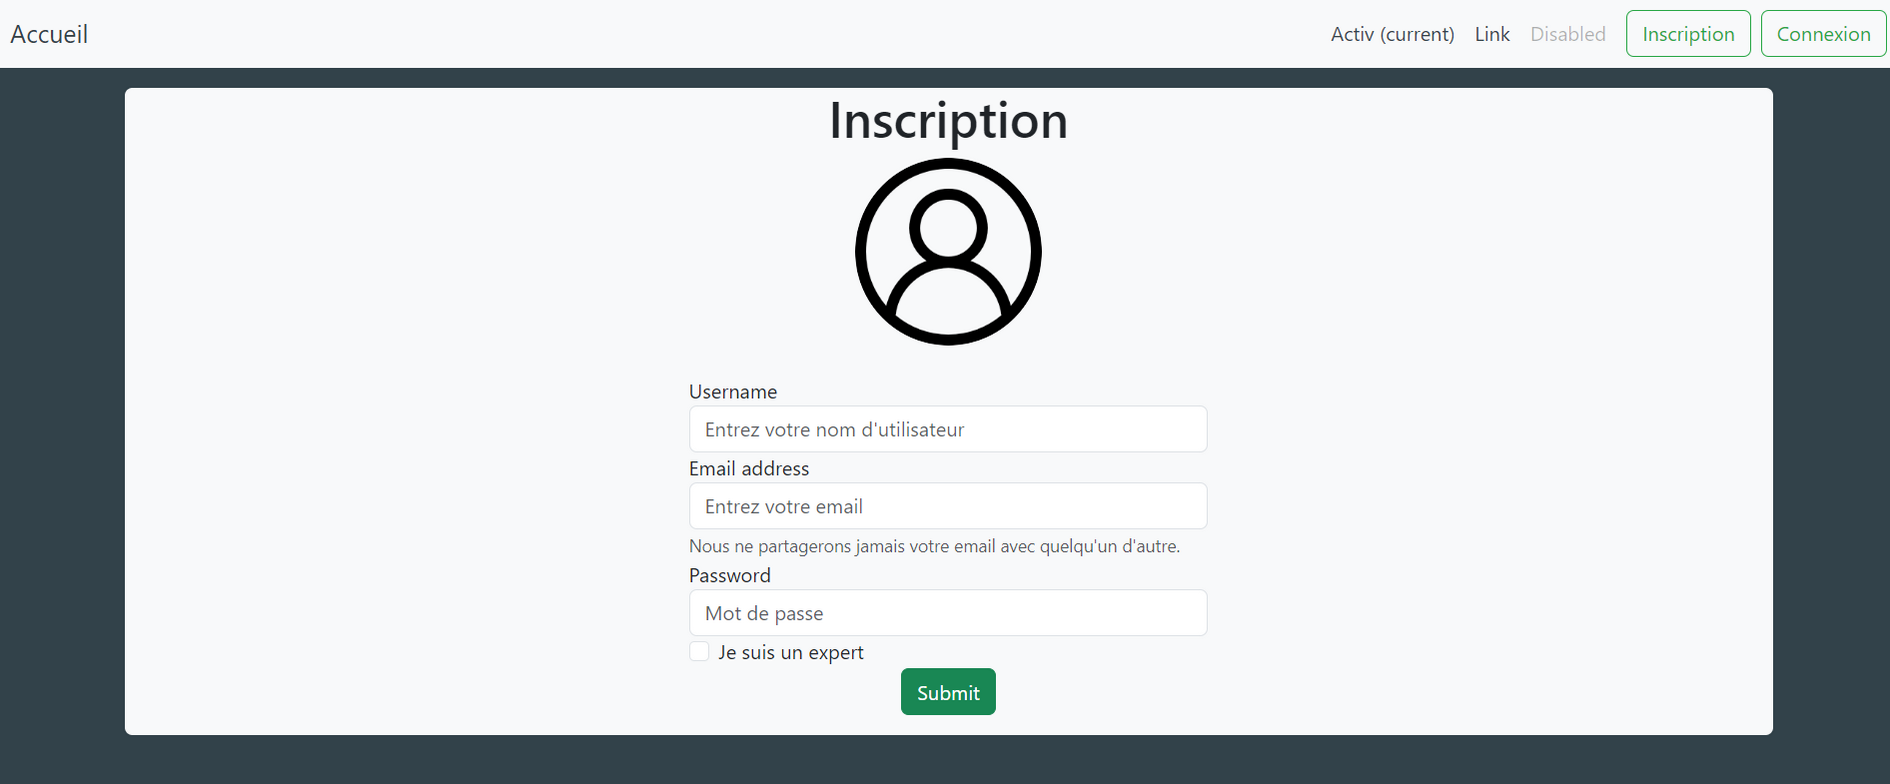
\includegraphics[width=\textwidth]{img_rmd/fig2.png}
\caption{Page de connexion}
\end{figure}

\newpage

\subsubsection{Accueil}\label{accueil}

L'accueil peut être défini comme l'élément central de cette interface
web, en effet c'est elle qui contient l'input permettant de passer sa
photo à l'intelligence artificielle en vue de la détection des espèces
de collemboles. Durant les premières semaines, une première version a
été réalisée (Fig 3). Cette version transmettait l'image importée à
YOLOv5 étant plus généraliste en attendant d'avoir le modèle entraîné.
Le choix de la version s'est orienté vers YOLOv5s car étant la plus
rapide, elle permet de faire plus de tests. Après avoir validé l'image à
analyser, le modèle charge et quand il fournit sa réponse l'utilisateur
est automatiquement redirigé vers une nouvelle page.

\begin{figure}[htbp]
\centering
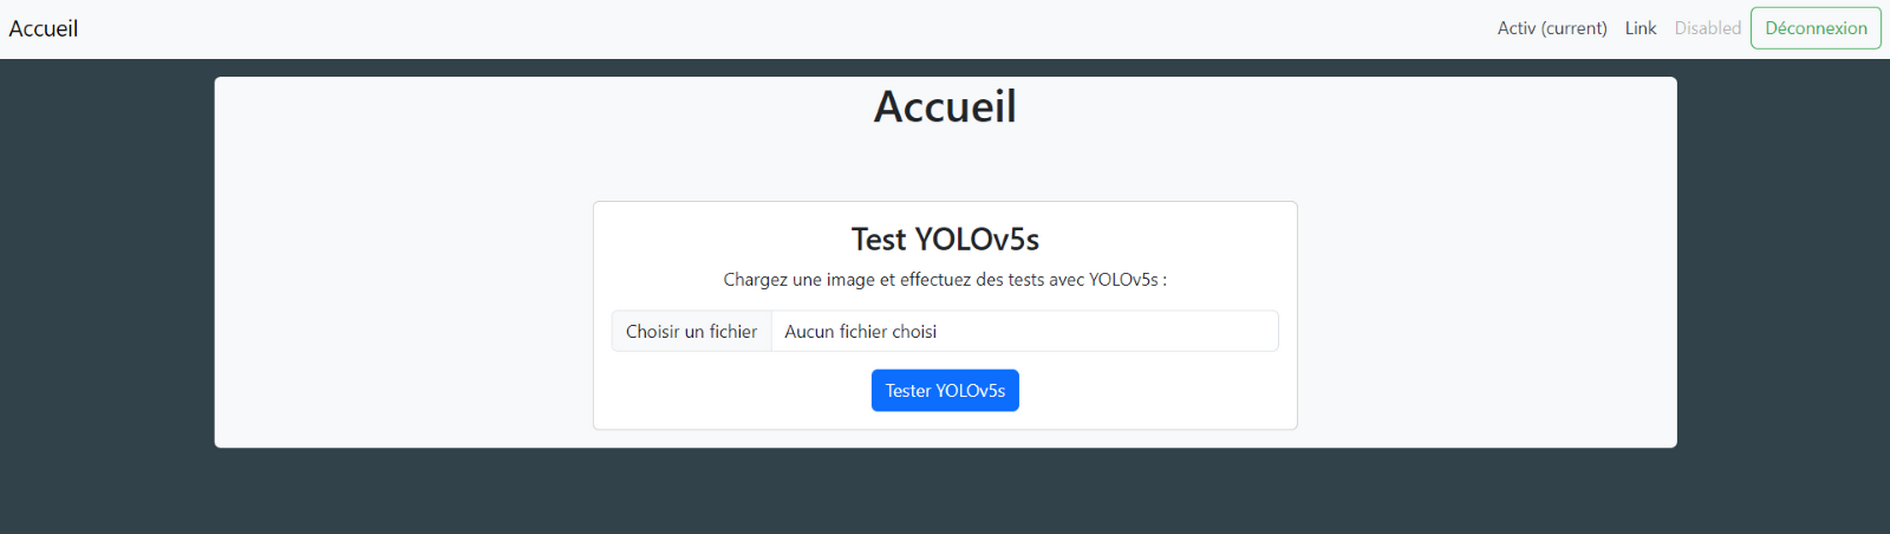
\includegraphics[width=\textwidth]{img_rmd/fig3.png}
\caption{Première version de la page d'accueil}
\end{figure}

Cette version de la page d'accueil manquait cruellement de vie et
d'accessibilité, un travail sur ces deux points a donc été fait pour
avoir une interface plus esthétique et permettant une meilleure
compréhension des images attendues dans le but d'effectuer une détection
précise grâce aux instructions écrites, mais aussi grâce au carrousel
montrant des images adaptées à la détection (Fig 4).

\begin{figure}[htbp]
\centering
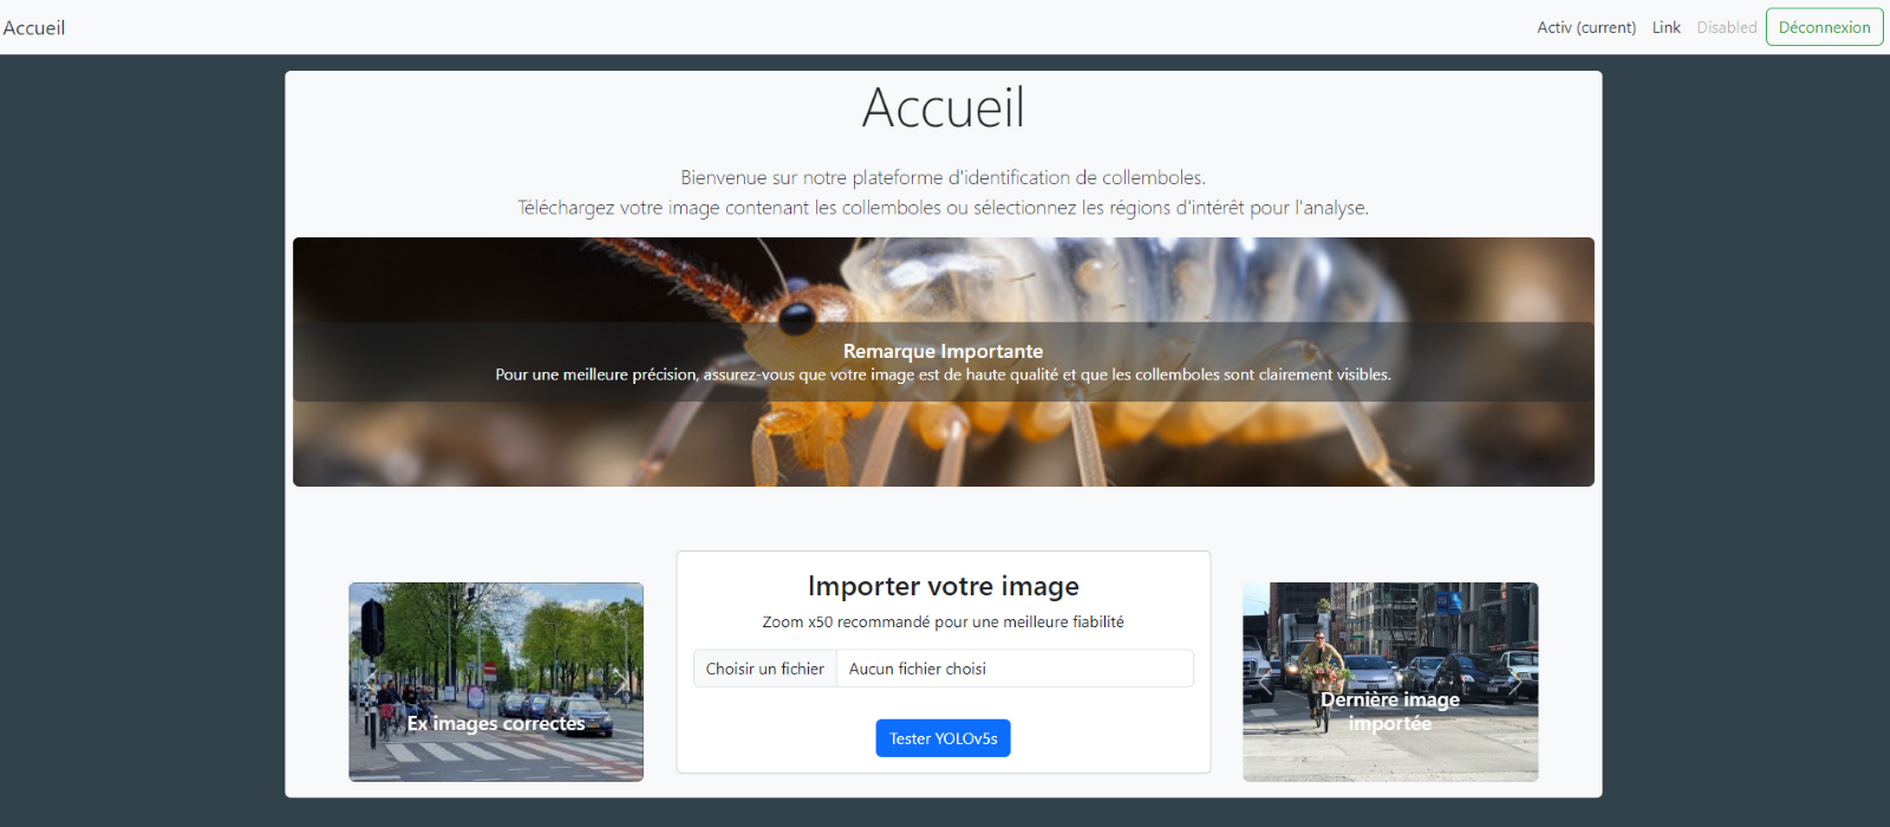
\includegraphics[width=\textwidth]{img_rmd/fig4.png}
\caption{Version améliorée de la page d'accueil}
\end{figure}

Pour accéder à toutes ces fonctionnalités, l'inscription est nécessaire,
ainsi s'il n'y a pas de session en cours, alors la page s'affichera avec
un affichage différent suggérant à l'utilisateur de se connecter pour
utiliser cette fonctionnalité (Fig 5).

\begin{figure}[htbp]
\centering
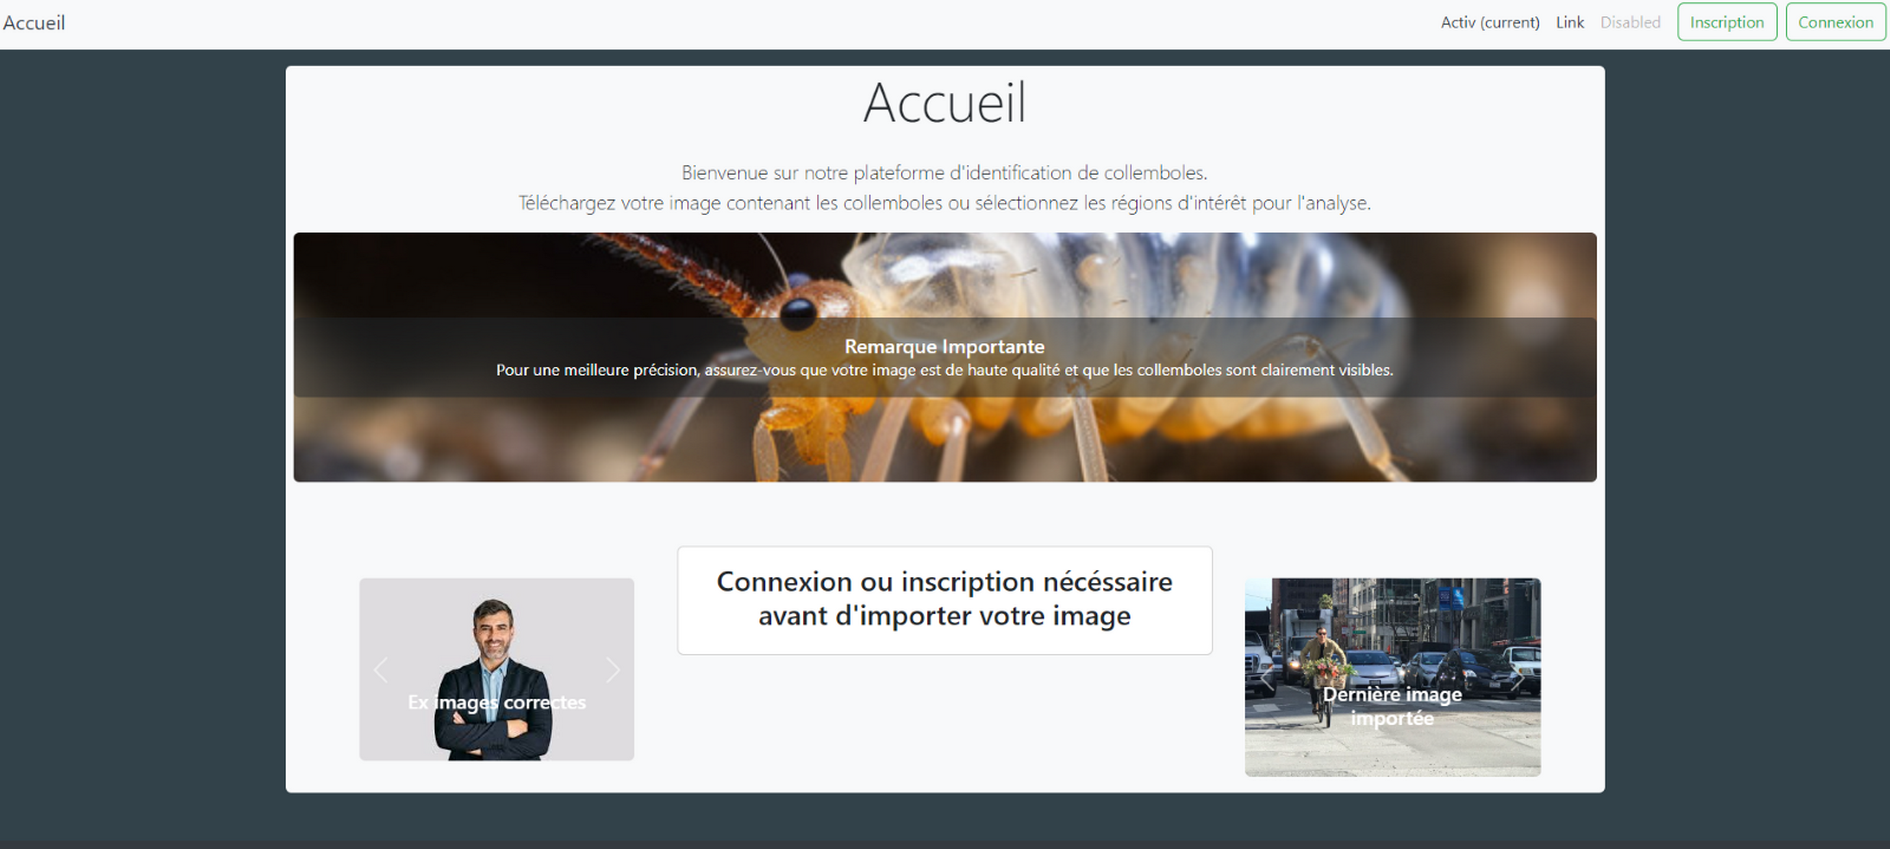
\includegraphics[width=\textwidth]{img_rmd/fig5.png}
\caption{Page d'accueil avec session inactive}
\end{figure}

\newpage

\subsubsection{Résultat de détection}\label{ruxe9sultat-de-duxe9tection}

Après la redirection depuis la page d'accueil, l'utilisateur arrive sur
cette page affichant les résultats de détection (Fig 6). On retrouve ici
l'image donnée par l'utilisateur accompagnée de boxes ajoutées grâce au
CSS qui récupère les coordonnées en pixels localisant les objets /
collemboles détectés par YOLOv5. Ces objets sont accompagnés de leur nom
ainsi qu'un chiffre unique à chacun. Une liste à gauche de l'image nous
permet d'observer les niveaux de confiance associés à chaque objet nous
donnant une indication précise quant à la précision de la classification
de l'objet en question. Aussi, un espace commentaire permet de
renseigner des informations sur la photo du type métadonnées (lieux /
date/\ldots) (Fig 7).

\begin{figure}[htbp]
\centering
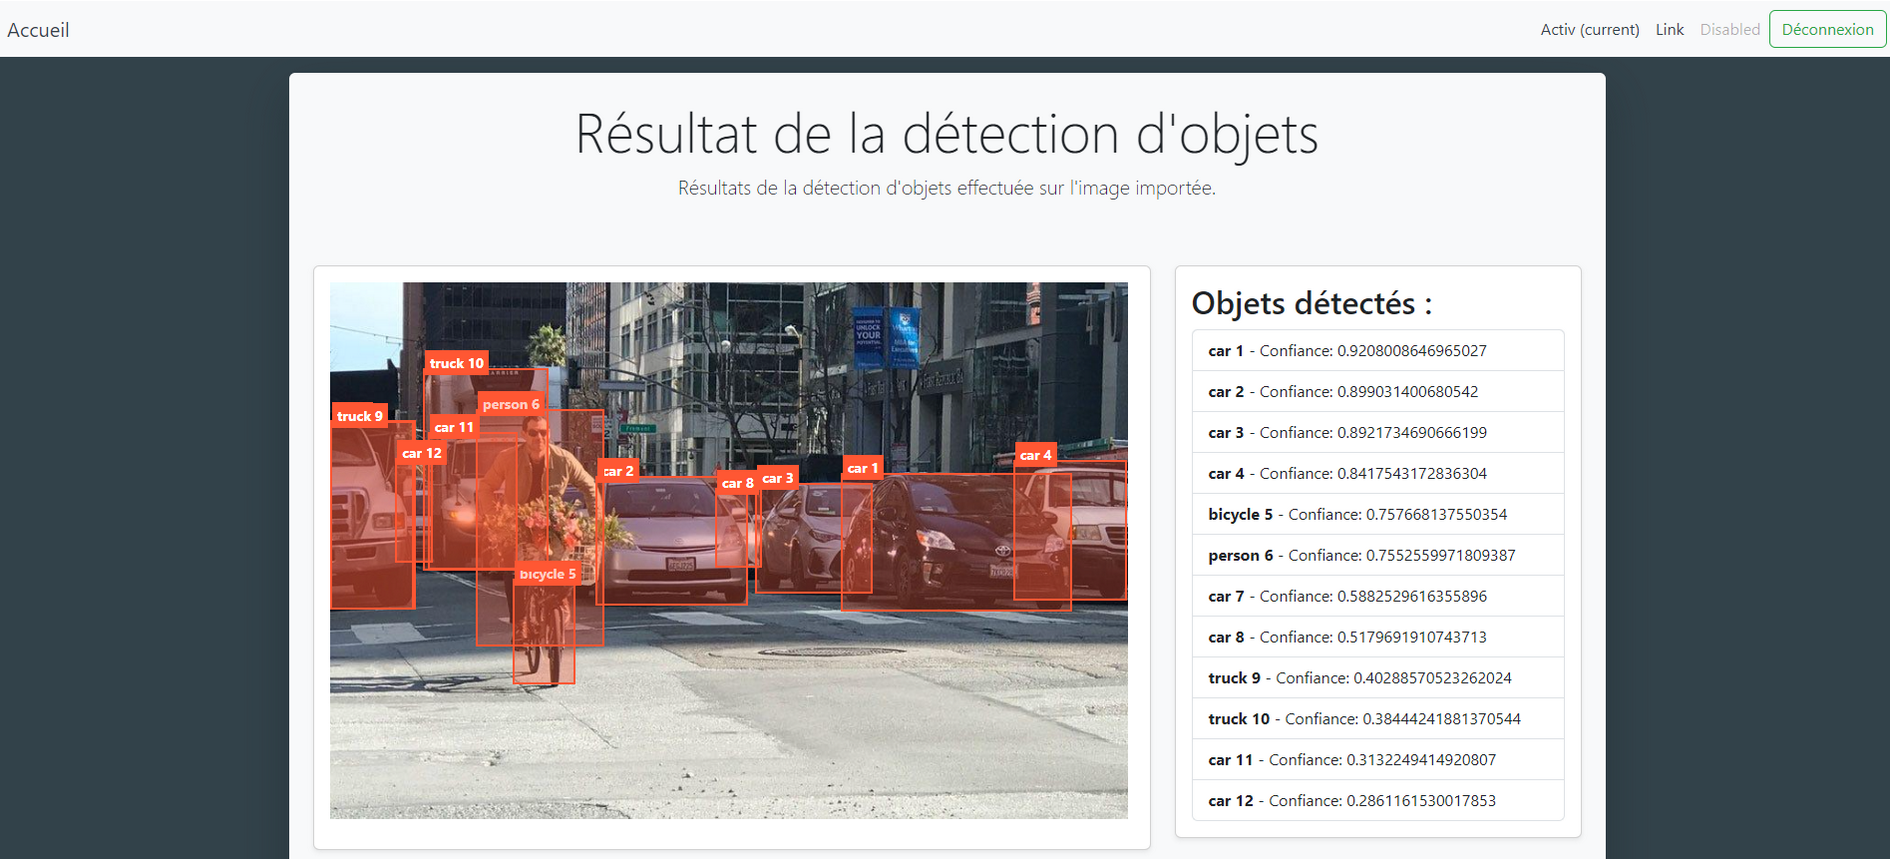
\includegraphics[width=\textwidth]{img_rmd/fig6.png}
\caption{Page des résultats de détection}
\end{figure}

\begin{figure}[htbp]
\centering

\includegraphics[width=\textwidth]{img_rmd/fig7.png}
\caption{Page des résultats avec commentaires}
\end{figure}

\newpage

\subsubsection{Annotation}\label{annotation}

La page Annotation a, elle aussi, un rôle prépondérant sur cette
interface web, elle permet de récupérer dans la base de données les
images sélectionnées par l'Active Learning pour les annoter avant
d'entraîner à nouveau le modèle. Dans le cadre d'annotations nécessitant
une réelle expertise du sujet, cette page est accessible uniquement au
profil ``Expert'' pour éviter le maximum d'annotations erronées et donc
indirectement éviter au modèle de fausses détections après entraînement.
Si le profil n'est pas expert, mais essaie d'accéder à cette page, alors
cette interface page apparaîtra.

\begin{figure}[htbp]
\centering
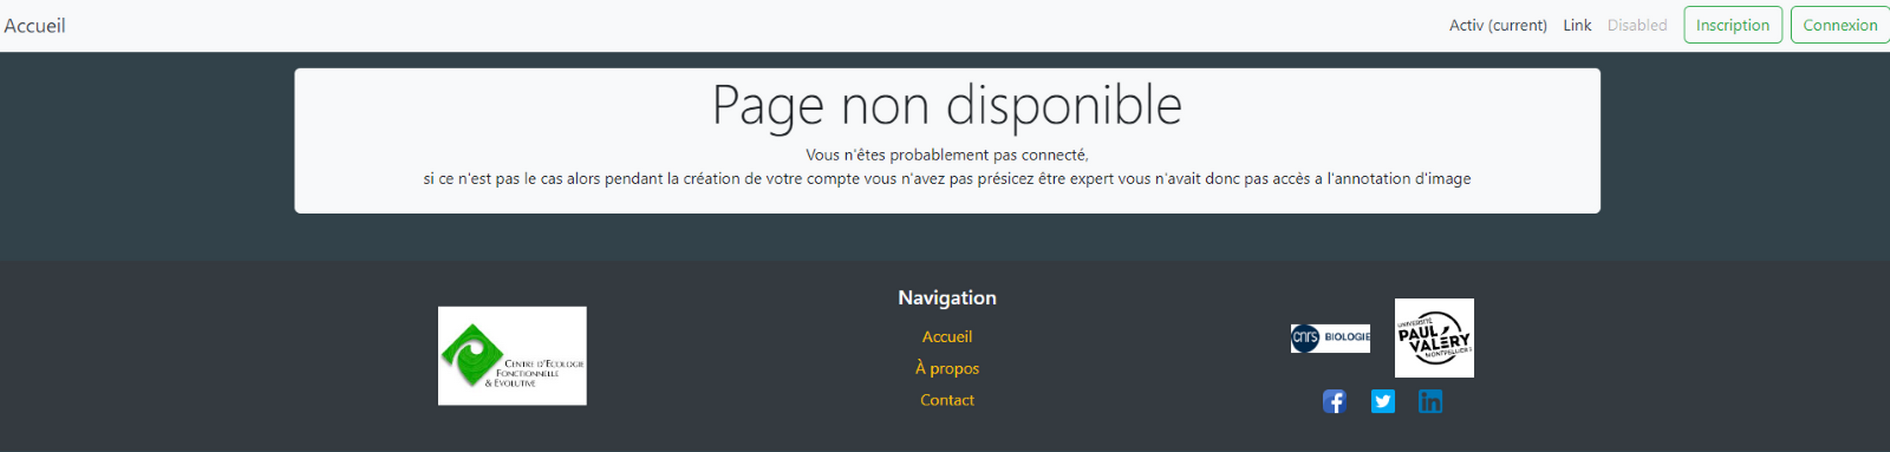
\includegraphics[width=\textwidth]{img_rmd/fig13.png}
\caption{Page d'annotation non experts}
\end{figure}

Le design et les fonctionnalités de cette page ont évolué au cours du
temps, mais le concept reste le même. L'utilisateur dispose d'une partie
à gauche de la page où il peut sélectionner des zones grâce à la souris
avant de leur donner un label. Ces zones seront répertoriées à droite de
la page permettant une relecture du label accompagné de ses coordonnées.
Pour envoyer ces annotations, il suffit à l'utilisateur d'appuyer sur le
bouton en bas de page. La première version de cette page garde tous ces
concepts, mais beaucoup de problèmes esthétiques et fonctionnels
(annotation par système de pop-up, les zones saisies ne sont pas
modifiables ou supprimables, problème de ratio pour les images, problème
d'affichage dans la liste des zones) (Fig 9, Fig 10).

\begin{figure}[htbp]
\centering
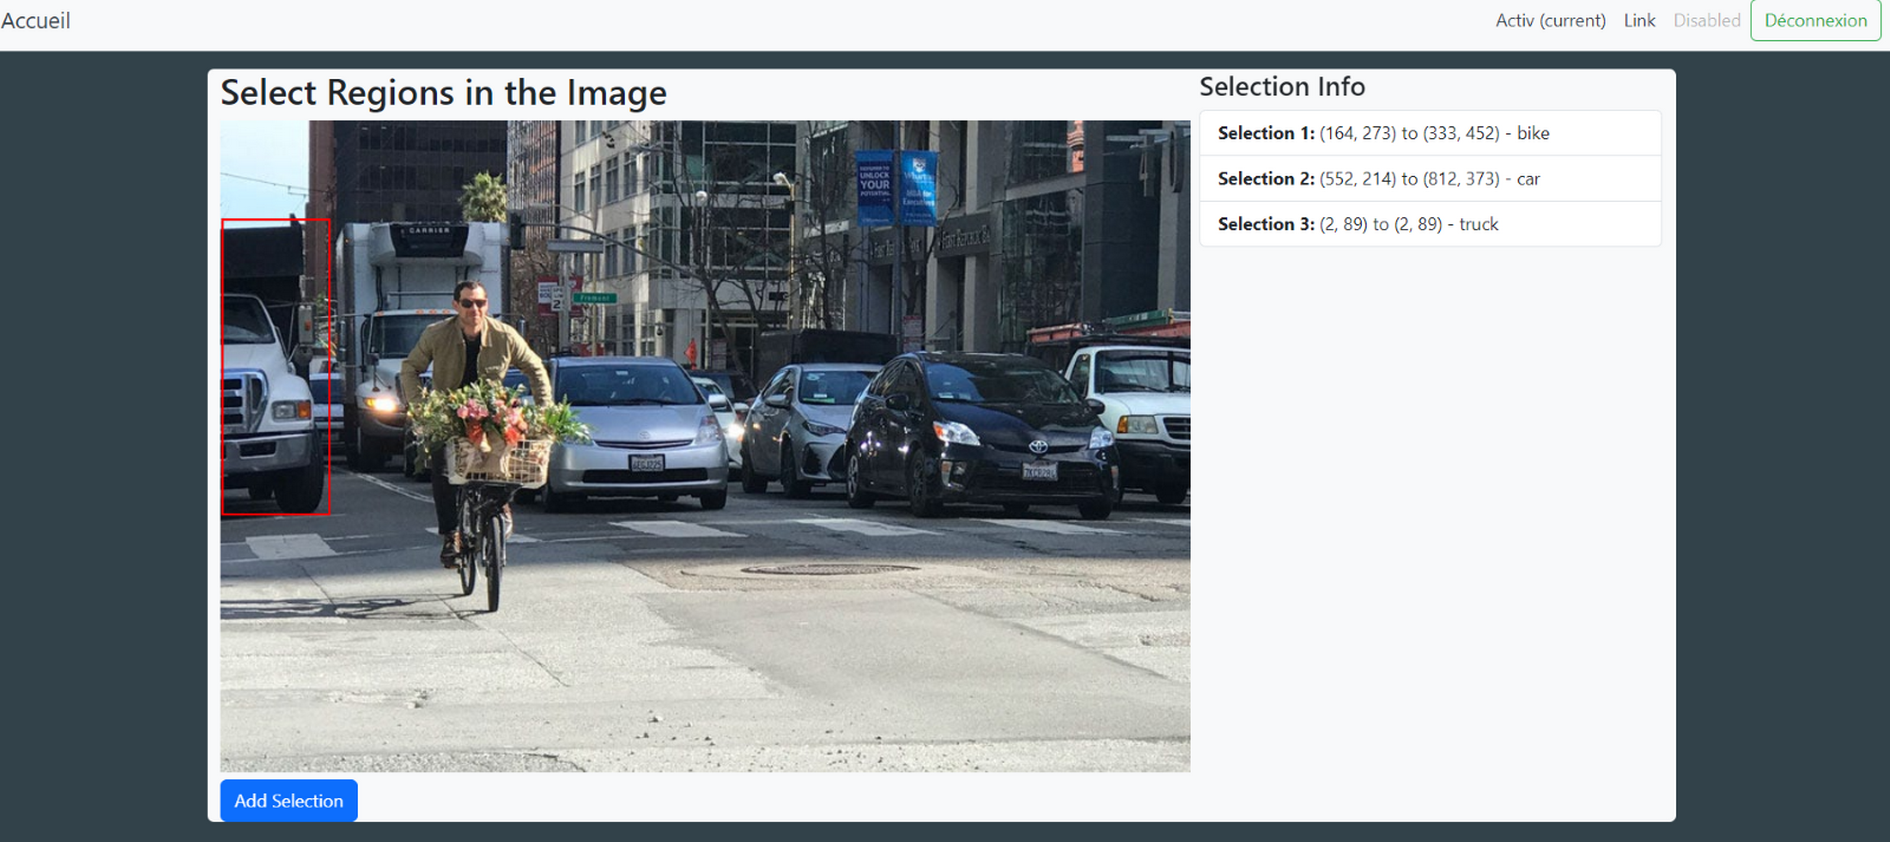
\includegraphics[width=\textwidth]{img_rmd/fig8.png}
\caption{Première version de la page d'annotation}
\end{figure}

\begin{figure}[htbp]
\centering
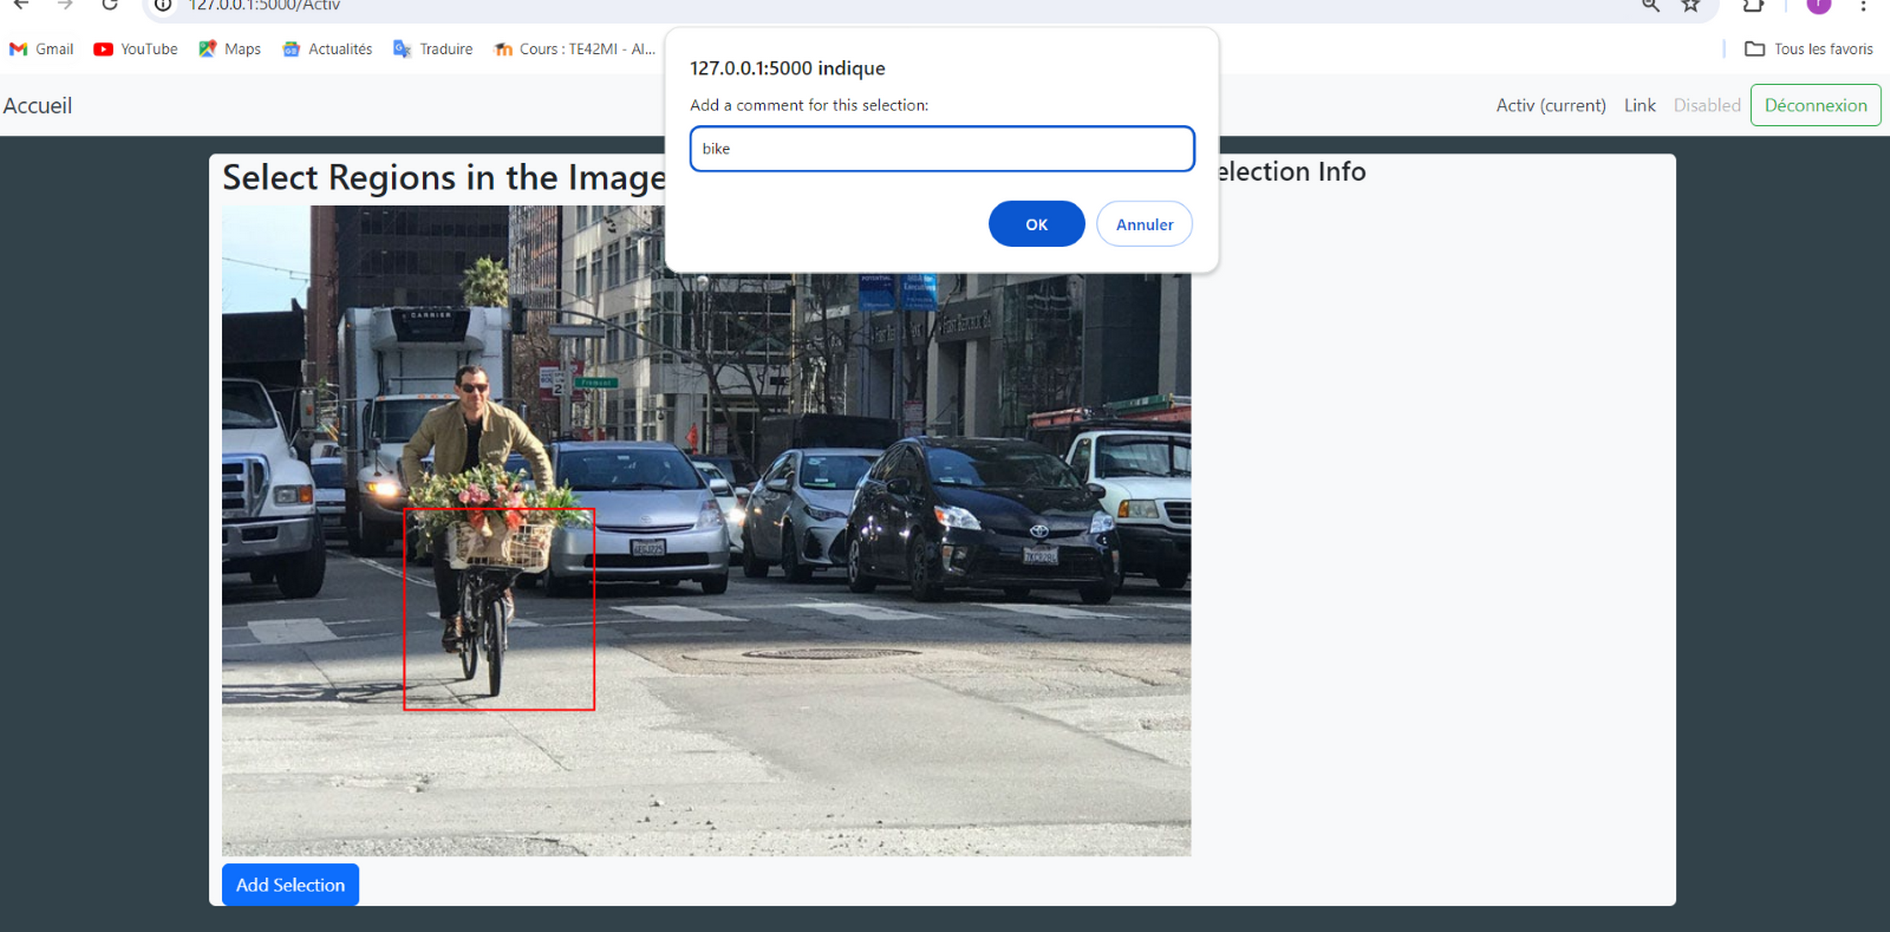
\includegraphics[width=\textwidth]{img_rmd/fig9.png}
\caption{Première version avec zones saisies}
\end{figure}

\newpage

Pour corriger tous les problèmes préalablement cités et améliorer
l'accessibilité ainsi que l'esthétique de la page, une nouvelle version
a été créée, étant beaucoup plus fonctionnelle et flexible pour
l'utilisateur (Fig 11, Fig 12).

\begin{figure}[htbp]
\centering
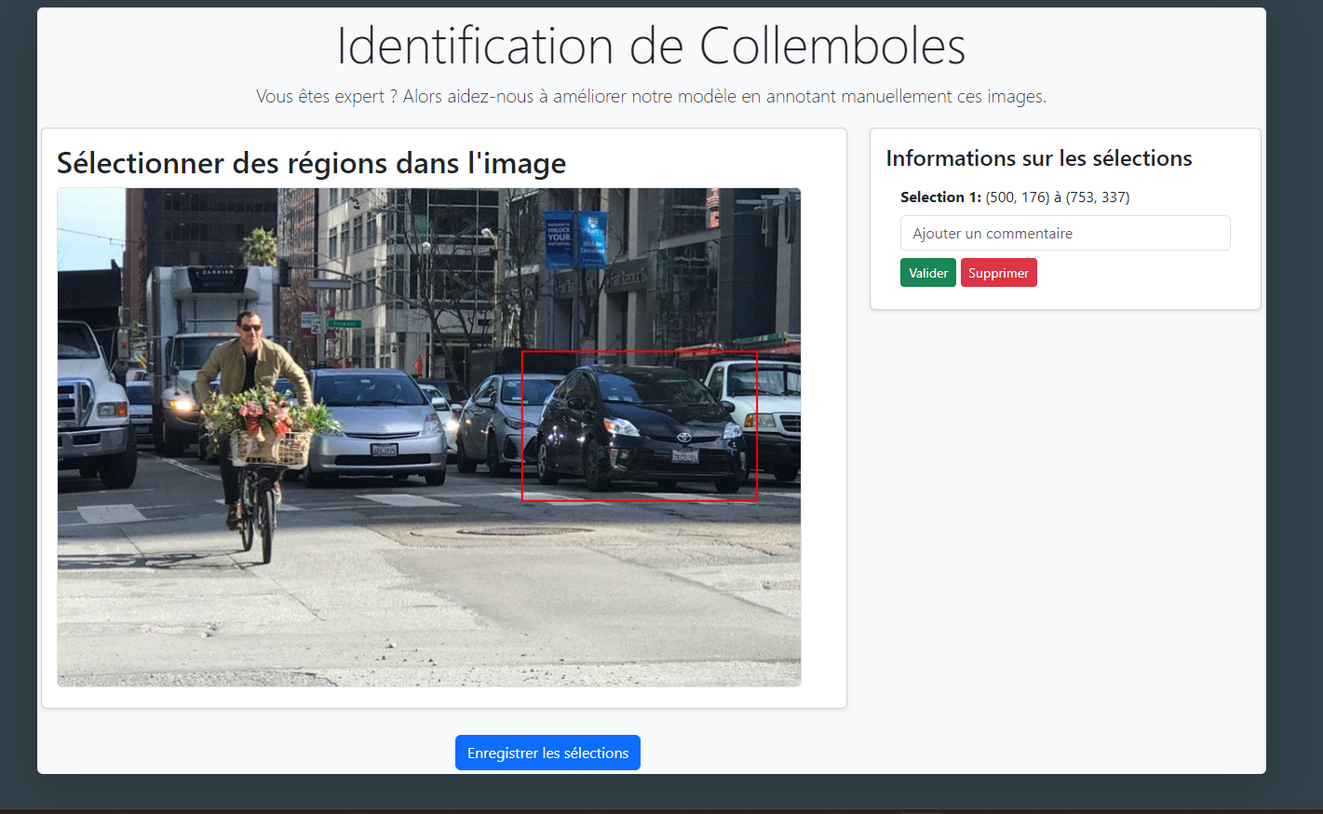
\includegraphics[width=\textwidth]{img_rmd/fig10.png}
\caption{Nouvelle version de la page d'annotation}
\end{figure}

\begin{figure}[htbp]
\centering
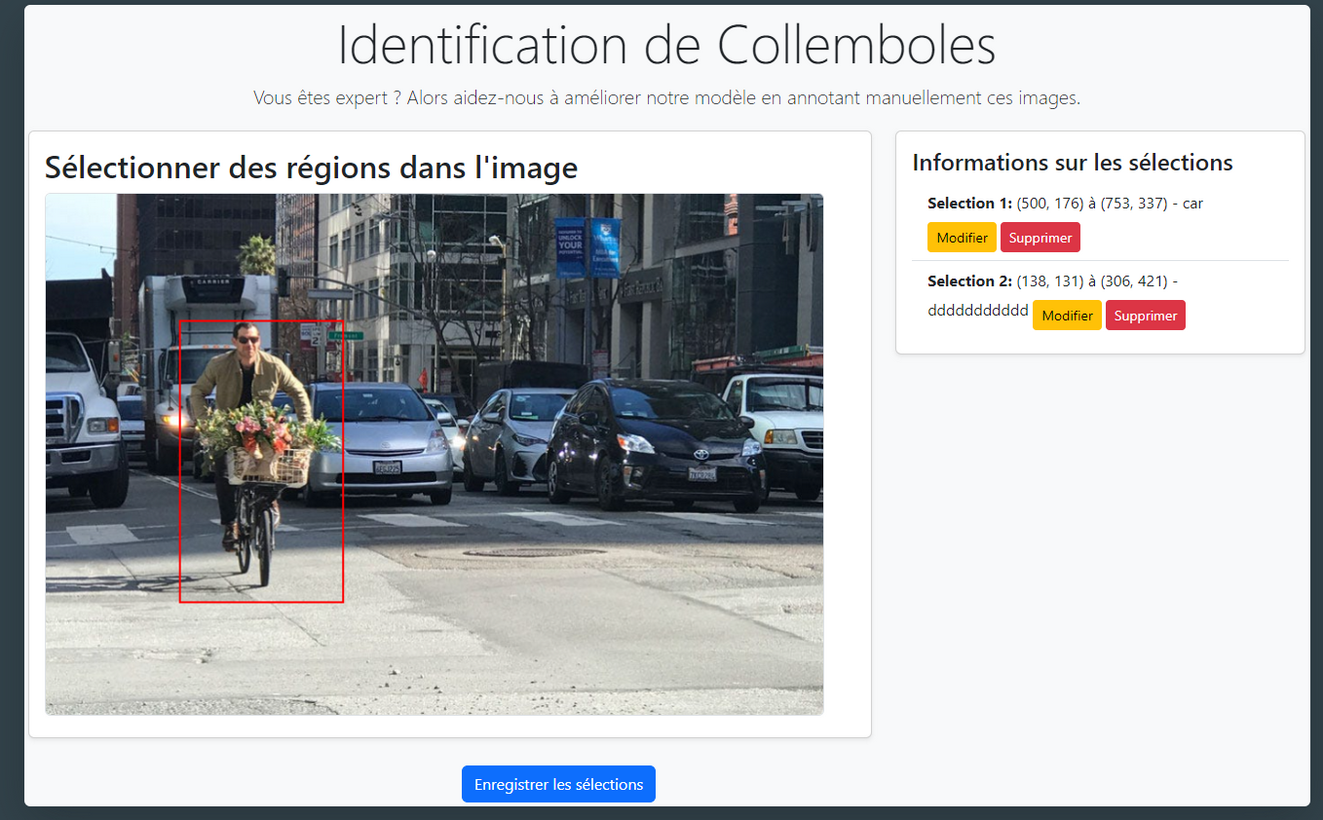
\includegraphics[width=\textwidth]{img_rmd/fig11.png}
\caption{Nouvelle version avec label modifiable }
\end{figure}

Un problème persistait quand même : les annotations semblaient peu
précises, car sans zone précise, certains éléments sont difficiles à
encadrer proprement. Le zoom semblait donc la meilleure option pour plus
de précision, l'ajout de boutons le permettant semblait de ce fait utile
ainsi qu'un zoom avec la souris (scroll) (Fig 13).

\begin{figure}[htbp]
\centering
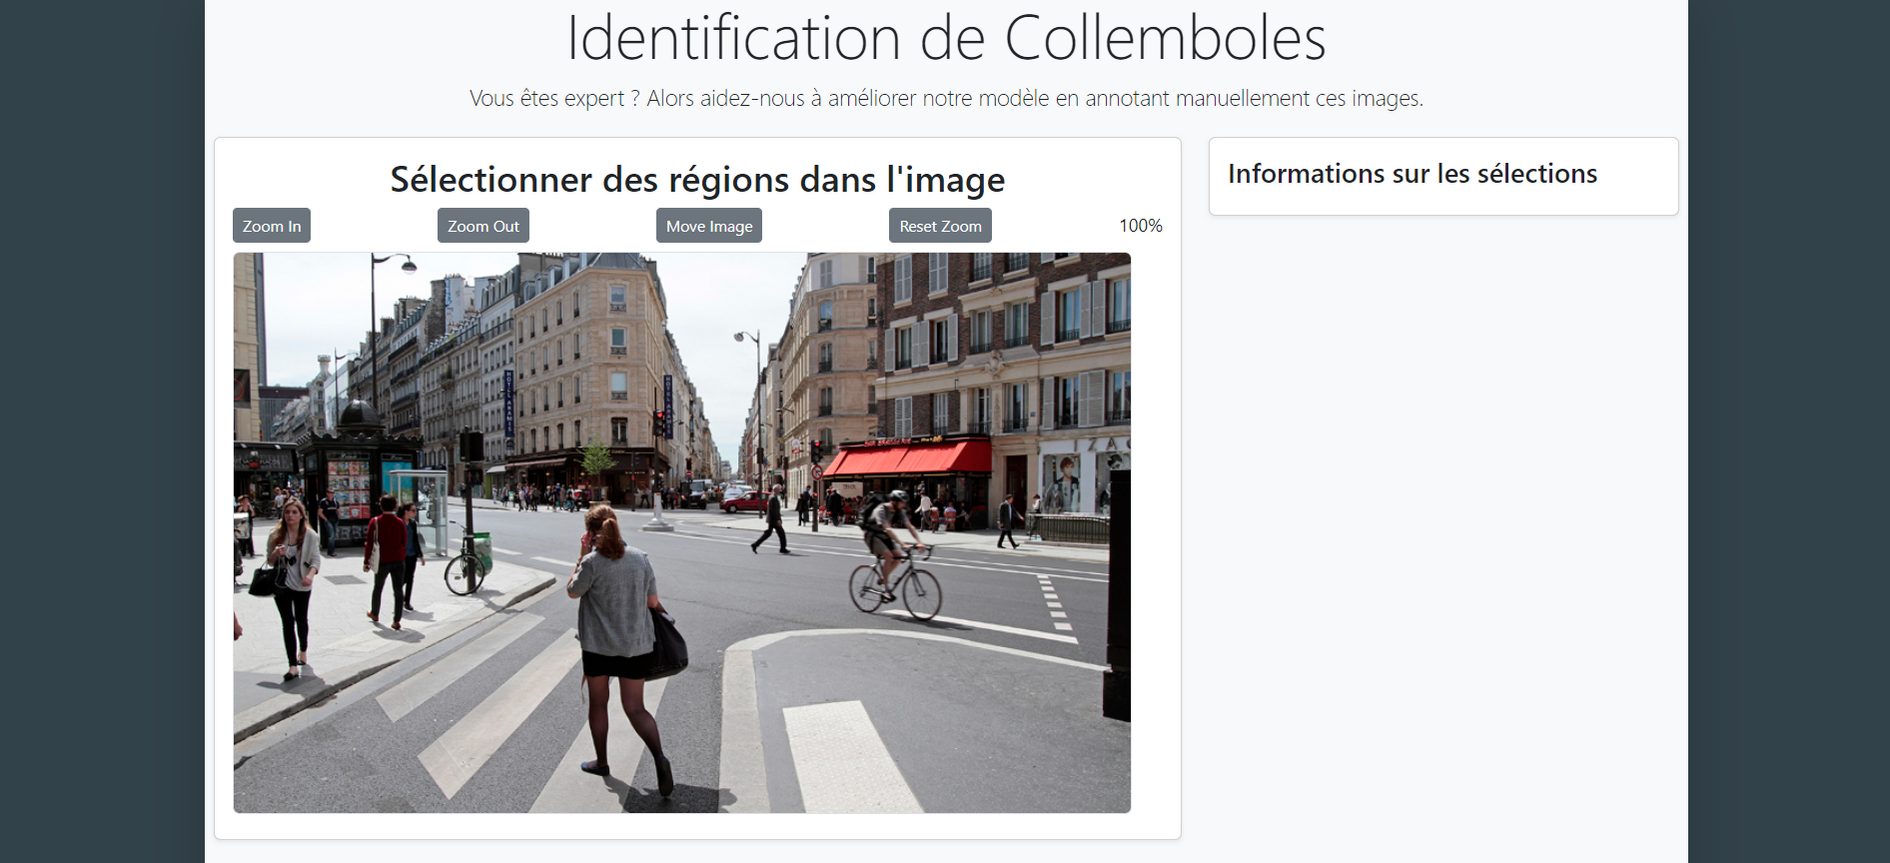
\includegraphics[width=\textwidth]{img_rmd/fig12.png}
\caption{Page d'annotation avec zoom}
\end{figure}

\newpage

\section{Base de données}\label{base-de-donnuxe9es}

\subsection{Descriptif des Tables}\label{descriptif-des-tables}

\subsubsection{Table~: clients}\label{table-clients}

\begin{longtable}[]{@{}
  >{\raggedright\arraybackslash}p{(\columnwidth - 6\tabcolsep) * \real{0.1610}}
  >{\raggedright\arraybackslash}p{(\columnwidth - 6\tabcolsep) * \real{0.2627}}
  >{\raggedright\arraybackslash}p{(\columnwidth - 6\tabcolsep) * \real{0.3051}}
  >{\raggedright\arraybackslash}p{(\columnwidth - 6\tabcolsep) * \real{0.2712}}@{}}
\toprule\noalign{}
\begin{minipage}[b]{\linewidth}\raggedright
Nom de la colonne
\end{minipage} & \begin{minipage}[b]{\linewidth}\raggedright
Type de données
\end{minipage} & \begin{minipage}[b]{\linewidth}\raggedright
Signification
\end{minipage} & \begin{minipage}[b]{\linewidth}\raggedright
Caractéristiques
\end{minipage} \\
\midrule\noalign{}
\endhead
\bottomrule\noalign{}
\endlastfoot
nom & Chaîne de caractère (varchar) & Nom du client & Clé primaire, non
nul, unique \\
email & Chaîne de caractère (varchar) & Adresse email du client & - \\
mdp & Chaîne de caractère (varchar) & Mot de passe crypté du client &
- \\
exp & Entier (tinyint) & expert ou non (0 ou 1) & Non nul \\
\end{longtable}

\subsubsection{Table: images}\label{table-images}

\begin{longtable}[]{@{}
  >{\raggedright\arraybackslash}p{(\columnwidth - 6\tabcolsep) * \real{0.1610}}
  >{\raggedright\arraybackslash}p{(\columnwidth - 6\tabcolsep) * \real{0.2627}}
  >{\raggedright\arraybackslash}p{(\columnwidth - 6\tabcolsep) * \real{0.3051}}
  >{\raggedright\arraybackslash}p{(\columnwidth - 6\tabcolsep) * \real{0.2712}}@{}}
\toprule\noalign{}
\begin{minipage}[b]{\linewidth}\raggedright
Nom de la colonne
\end{minipage} & \begin{minipage}[b]{\linewidth}\raggedright
Type de données
\end{minipage} & \begin{minipage}[b]{\linewidth}\raggedright
Signification
\end{minipage} & \begin{minipage}[b]{\linewidth}\raggedright
Caractéristiques
\end{minipage} \\
\midrule\noalign{}
\endhead
\bottomrule\noalign{}
\endlastfoot
id & Entier (integer) & Identifiant unique de l'image & Clé primaire,
non nul, unique \\
username & Chaîne de caractère (varchar) & Nom d'utilisateur associé à
l'image & Non nul \\
url & Chaîne de caractère (varchar) & URL de l'image & Non nul \\
commentaire & Texte (text) & Commentaire sur l'image(lieux/date) & - \\
\end{longtable}

\subsubsection{Table: img\_annot}\label{table-img_annot}

\begin{longtable}[]{@{}
  >{\raggedright\arraybackslash}p{(\columnwidth - 6\tabcolsep) * \real{0.1610}}
  >{\raggedright\arraybackslash}p{(\columnwidth - 6\tabcolsep) * \real{0.2627}}
  >{\raggedright\arraybackslash}p{(\columnwidth - 6\tabcolsep) * \real{0.3051}}
  >{\raggedright\arraybackslash}p{(\columnwidth - 6\tabcolsep) * \real{0.2712}}@{}}
\toprule\noalign{}
\begin{minipage}[b]{\linewidth}\raggedright
Nom de la colonne
\end{minipage} & \begin{minipage}[b]{\linewidth}\raggedright
Type de données
\end{minipage} & \begin{minipage}[b]{\linewidth}\raggedright
Signification
\end{minipage} & \begin{minipage}[b]{\linewidth}\raggedright
Caractéristiques
\end{minipage} \\
\midrule\noalign{}
\endhead
\bottomrule\noalign{}
\endlastfoot
img\_id & Entier (integer) & Identifiant unique de l'image & Clé
primaire, non nul, unique \\
img\_url & Chaîne de caractère (varchar) & URL de l'image & Non nul \\
user & Chaîne de caractère (varchar) & Nom d'utilisateur associé à
l'image & Non nul \\
label & Chaîne de caractère (varchar) & label/coordonnées associées à
l'image & Peut être vide \\
\end{longtable}

\newpage

\section{Deep Learning}\label{deep-learning}

\subsection{Implémentation du
modèle}\label{impluxe9mentation-du-moduxe8le}

Avant de pouvoir procéder à toute détection, il est nécessaire
d'implémenter un modèle dans le code. Comme mentionné précédemment, le
modèle utilisé était ``Yolov5s'', cependant il n'était pas encore
entraîné. Pour utiliser ce modèle, plusieurs fonctions sont nécessaires
pour charger et interpréter les images dans la fonction ``detect''.

\begin{Shaded}
\begin{Highlighting}[]
\AttributeTok{@app.route}\NormalTok{(}\StringTok{\textquotesingle{}/detect\textquotesingle{}}\NormalTok{, methods}\OperatorTok{=}\NormalTok{[}\StringTok{\textquotesingle{}POST\textquotesingle{}}\NormalTok{])}
\KeywordTok{def}\NormalTok{ detect\_img():}
    \ControlFlowTok{if}\NormalTok{ request.method }\OperatorTok{==} \StringTok{\textquotesingle{}POST\textquotesingle{}}\NormalTok{:}
\NormalTok{        model }\OperatorTok{=}\NormalTok{ load\_models()  }\CommentTok{\# Charger le modèle YOLOv5}
        \ControlFlowTok{if} \StringTok{\textquotesingle{}image\textquotesingle{}} \KeywordTok{in}\NormalTok{ request.files:}
\NormalTok{            image\_file }\OperatorTok{=}\NormalTok{ request.files[}\StringTok{\textquotesingle{}image\textquotesingle{}}\NormalTok{]}
            \ControlFlowTok{if}\NormalTok{ image\_file.filename }\OperatorTok{==} \StringTok{\textquotesingle{}\textquotesingle{}}\NormalTok{:}
                \ControlFlowTok{return} \StringTok{"Aucun fichier sélectionné"}
            
\NormalTok{            image\_path }\OperatorTok{=}\NormalTok{ os.path.join(app.config[}\StringTok{\textquotesingle{}UPLOAD\_FOLDER\textquotesingle{}}\NormalTok{], image\_file.filename)}
\NormalTok{            image\_file.save(image\_path)}

            \CommentTok{\# Charger l\textquotesingle{}image avec PIL et la convertir en ndarray OpenCV}
\NormalTok{            img }\OperatorTok{=}\NormalTok{ Image.}\BuiltInTok{open}\NormalTok{(image\_file.stream).convert(}\StringTok{"RGB"}\NormalTok{)}
\NormalTok{            img\_cv2 }\OperatorTok{=}\NormalTok{ cv2.cvtColor(np.array(img), cv2.COLOR\_RGB2BGR)}

            \CommentTok{\# Effectuer la détection avec YOLOv5s}
\NormalTok{            results }\OperatorTok{=}\NormalTok{ model(img\_cv2)}

            \CommentTok{\# Récupérer les résultats de détection au format JSON}
\NormalTok{            detections }\OperatorTok{=}\NormalTok{ results.pandas().xyxy[}\DecValTok{0}\NormalTok{].to\_dict(orient}\OperatorTok{=}\StringTok{\textquotesingle{}records\textquotesingle{}}\NormalTok{)}
\NormalTok{            img\_with\_boxes }\OperatorTok{=}\NormalTok{ results.render()  }
            \CommentTok{\# Récupérer l\textquotesingle{}image avec les boîtes de détection}

            \CommentTok{\# Convertir l\textquotesingle{}image en bytes}
\NormalTok{            img\_byte\_array }\OperatorTok{=}\NormalTok{ BytesIO()}
\NormalTok{            img.save(img\_byte\_array, }\BuiltInTok{format}\OperatorTok{=}\StringTok{\textquotesingle{}JPEG\textquotesingle{}}\NormalTok{)}
\NormalTok{            img\_data }\OperatorTok{=}\NormalTok{ img\_byte\_array.getvalue()}

            \CommentTok{\# Encoder les données d\textquotesingle{}image en base64}
\NormalTok{            img\_base64 }\OperatorTok{=}\NormalTok{ base64.b64encode(img\_data).decode(}\StringTok{\textquotesingle{}utf{-}8\textquotesingle{}}\NormalTok{)}
\NormalTok{            image\_url }\OperatorTok{=}\NormalTok{ url\_for(}\StringTok{\textquotesingle{}static\textquotesingle{}}\NormalTok{, filename}\OperatorTok{=}\StringTok{\textquotesingle{}img\_load/\textquotesingle{}} \OperatorTok{+}\NormalTok{ image\_file.filename)}

            \CommentTok{\# Vérifier si l\textquotesingle{}image doit être enregistrée}
            \ControlFlowTok{if}\NormalTok{ should\_save\_image(results, threshold\_confidence}\OperatorTok{=}\FloatTok{0.5}\NormalTok{):}
\NormalTok{                nom }\OperatorTok{=}\NormalTok{ session[}\StringTok{\textquotesingle{}username\textquotesingle{}}\NormalTok{]}
                \ControlFlowTok{if}\NormalTok{ ajt\_img(image\_url, nom):}
                    \BuiltInTok{print}\NormalTok{(}\StringTok{"\textless{}script\textgreater{}alert(\textquotesingle{}img!\textquotesingle{}); window.location.href=\textquotesingle{}/\textquotesingle{};\textless{}/script\textgreater{}"}\NormalTok{)}
                \ControlFlowTok{else}\NormalTok{:}
                    \BuiltInTok{print}\NormalTok{(}\StringTok{"\textless{}script\textgreater{}alert(\textquotesingle{}not!\textquotesingle{}); window.location.href=\textquotesingle{}/\textquotesingle{};\textless{}/script\textgreater{}"}\NormalTok{)}
            
            \CommentTok{\# Retourner le template result.html avec les données de détection}
            \ControlFlowTok{return}\NormalTok{ render\_template(}\StringTok{\textquotesingle{}result.html\textquotesingle{}}\NormalTok{, detections}\OperatorTok{=}\NormalTok{detections,}
\NormalTok{            image}\OperatorTok{=}\NormalTok{img\_base64, img\_url}\OperatorTok{=}\NormalTok{image\_url)}
        \ControlFlowTok{else}\NormalTok{:}
            \ControlFlowTok{return} \StringTok{"Aucun fichier trouvé dans la requête"}
\end{Highlighting}
\end{Shaded}

\subsection{Active Learning}\label{active-learning}

Comme discuté dans la partie précédente sur le développement web,
l'Active Learning est essentiel pour améliorer le modèle. Les images
pertinentes sont enregistrées dans la base de données pour entraîner et
améliorer le modèle. Avant l'implémentation d'un Active Learning plus
avancé, les images contenant plus de 3 objets avec un score de confiance
inférieur à 0.40 sont automatiquement sauvegardées dans une nouvelle
table de la base de données (img\_annot). (Fig 2)

\begin{Shaded}
\begin{Highlighting}[]
\KeywordTok{def}\NormalTok{ should\_save\_image(results, threshold\_confidence}\OperatorTok{=}\FloatTok{0.5}\NormalTok{):}
    \CommentTok{\# Examinez les résultats de YOLO pour déterminer si l\textquotesingle{}image doit être enregistrée}
\NormalTok{    detections }\OperatorTok{=}\NormalTok{ results.pandas().xyxy[}\DecValTok{0}\NormalTok{].to\_dict(orient}\OperatorTok{=}\StringTok{\textquotesingle{}records\textquotesingle{}}\NormalTok{)}
\NormalTok{    max\_confidence }\OperatorTok{=} \BuiltInTok{min}\NormalTok{(d[}\StringTok{\textquotesingle{}confidence\textquotesingle{}}\NormalTok{] }\ControlFlowTok{for}\NormalTok{ d }\KeywordTok{in}\NormalTok{ detections)}
    \ControlFlowTok{return}\NormalTok{ max\_confidence }\OperatorTok{\textless{}}\NormalTok{ threshold\_confidence}
\end{Highlighting}
\end{Shaded}

\subsection{Fine Tuning}\label{fine-tuning}

En l'état actuel des choses, l'interface web fonctionne correctement et
contient tous les éléments demandés et nécessaires à son bon
fonctionnement. Les utilisateurs peuvent importer des images, les plus
intéressantes sont sauvegardées dans la base de données (``Active
Learning''), puis les images sont annotées par des experts et
réintroduites dans la base de données avec les coordonnées et les
étiquettes ajoutées. Cependant, pour l'instant, le modèle ne s'entraîne
pas automatiquement. Pour atteindre cet objectif, il faut se concentrer
sur la partie ``Fine Tuning''. Pour cela, beaucoup de recherches sont
nécessaires car ces notions n'ont jamais été abordées en cours.

Pour crée le fine tuning, cela se découpe en plusieurs parties : les
images sélectionnées doivent être déplacées dans les dossiers du modèle
YOLO utilisé, c'est-à-dire dans ``val'' et ``train'' (fig 13). À chaque
image est associé un fichier TXT contenant les annotations effectuées
par les utilisateurs. Comme mentionné précédemment, les annotations
faites sont associées à des coordonnées et à des labels. Cependant, YOLO
étant un modèle de recherche sur images, il fonctionne grâce à un
système d'ancrages. Ainsi, les coordonnées en pixels et les labels
doivent être convertis pour répondre aux attentes de YOLO. Pour
convertir ces coordonnées, il faut récupérer les informations dans la
base de données, puis les transformer et créer les fichiers TXT au
format YOLO.

\begin{Shaded}
\begin{Highlighting}[]
\KeywordTok{def}\NormalTok{ ensure\_directory\_exists(directory):}
    \ControlFlowTok{if} \KeywordTok{not}\NormalTok{ os.path.exists(directory):}
\NormalTok{        os.makedirs(directory)}

\KeywordTok{def}\NormalTok{ split\_dataset(source\_dir, annotations\_dir, train\_dir, val\_dir, test\_dir}
\NormalTok{                          , train\_ratio}\OperatorTok{=}\FloatTok{0.7}\NormalTok{, val\_ratio}\OperatorTok{=}\FloatTok{0.2}\NormalTok{, test\_ratio}\OperatorTok{=}\FloatTok{0.1}\NormalTok{):}

\NormalTok{    images }\OperatorTok{=}\NormalTok{ [f }\ControlFlowTok{for}\NormalTok{ f }\KeywordTok{in}\NormalTok{ os.listdir(source\_dir) }\ControlFlowTok{if}\NormalTok{ f.endswith(}\StringTok{\textquotesingle{}.jpg\textquotesingle{}}\NormalTok{)]}
\NormalTok{    random.shuffle(images)}

\NormalTok{    train\_cutoff }\OperatorTok{=} \BuiltInTok{int}\NormalTok{(}\BuiltInTok{len}\NormalTok{(images) }\OperatorTok{*}\NormalTok{ train\_ratio)}
\NormalTok{    val\_cutoff }\OperatorTok{=}\NormalTok{ train\_cutoff }\OperatorTok{+} \BuiltInTok{int}\NormalTok{(}\BuiltInTok{len}\NormalTok{(images) }\OperatorTok{*}\NormalTok{ val\_ratio)}

\NormalTok{    train\_images }\OperatorTok{=}\NormalTok{ images[:train\_cutoff]}
\NormalTok{    val\_images }\OperatorTok{=}\NormalTok{ images[train\_cutoff:val\_cutoff]}
\NormalTok{    test\_images }\OperatorTok{=}\NormalTok{ images[val\_cutoff:]}

    \CommentTok{\# Ensure directories exist}
\NormalTok{    ensure\_directory\_exists(train\_dir)}
\NormalTok{    ensure\_directory\_exists(val\_dir)}
\NormalTok{    ensure\_directory\_exists(test\_dir)}

    \ControlFlowTok{for}\NormalTok{ img }\KeywordTok{in}\NormalTok{ train\_images:}
\NormalTok{        shutil.copy(os.path.join(source\_dir, img), os.path.join(train\_dir, img))}
\NormalTok{        txt\_file }\OperatorTok{=}\NormalTok{ img.replace(}\StringTok{\textquotesingle{}.jpg\textquotesingle{}}\NormalTok{, }\StringTok{\textquotesingle{}.txt\textquotesingle{}}\NormalTok{)}
\NormalTok{        src\_txt\_path }\OperatorTok{=}\NormalTok{ os.path.join(annotations\_dir, txt\_file)}
\NormalTok{        dst\_txt\_path }\OperatorTok{=}\NormalTok{ os.path.join(train\_dir, txt\_file)}
        \ControlFlowTok{if}\NormalTok{ os.path.exists(src\_txt\_path):}
\NormalTok{            shutil.copy(src\_txt\_path, dst\_txt\_path)}
            \BuiltInTok{print}\NormalTok{(}\SpecialStringTok{f"Copied }\SpecialCharTok{\{}\NormalTok{src\_txt\_path}\SpecialCharTok{\}}\SpecialStringTok{ to }\SpecialCharTok{\{}\NormalTok{dst\_txt\_path}\SpecialCharTok{\}}\SpecialStringTok{"}\NormalTok{)}

    \ControlFlowTok{for}\NormalTok{ img }\KeywordTok{in}\NormalTok{ val\_images:}
\NormalTok{        shutil.copy(os.path.join(source\_dir, img), os.path.join(val\_dir, img))}
\NormalTok{        txt\_file }\OperatorTok{=}\NormalTok{ img.replace(}\StringTok{\textquotesingle{}.jpg\textquotesingle{}}\NormalTok{, }\StringTok{\textquotesingle{}.txt\textquotesingle{}}\NormalTok{)}
\NormalTok{        src\_txt\_path }\OperatorTok{=}\NormalTok{ os.path.join(annotations\_dir, txt\_file)}
\NormalTok{        dst\_txt\_path }\OperatorTok{=}\NormalTok{ os.path.join(val\_dir, txt\_file)}
        \ControlFlowTok{if}\NormalTok{ os.path.exists(src\_txt\_path):}
\NormalTok{            shutil.copy(src\_txt\_path, dst\_txt\_path)}
            \BuiltInTok{print}\NormalTok{(}\SpecialStringTok{f"Copied }\SpecialCharTok{\{}\NormalTok{src\_txt\_path}\SpecialCharTok{\}}\SpecialStringTok{ to }\SpecialCharTok{\{}\NormalTok{dst\_txt\_path}\SpecialCharTok{\}}\SpecialStringTok{"}\NormalTok{)}

    \ControlFlowTok{for}\NormalTok{ img }\KeywordTok{in}\NormalTok{ test\_images:}
\NormalTok{        shutil.copy(os.path.join(source\_dir, img), os.path.join(test\_dir, img))}
\NormalTok{        txt\_file }\OperatorTok{=}\NormalTok{ img.replace(}\StringTok{\textquotesingle{}.jpg\textquotesingle{}}\NormalTok{, }\StringTok{\textquotesingle{}.txt\textquotesingle{}}\NormalTok{)}
\NormalTok{        src\_txt\_path }\OperatorTok{=}\NormalTok{ os.path.join(annotations\_dir, txt\_file)}
\NormalTok{        dst\_txt\_path }\OperatorTok{=}\NormalTok{ os.path.join(test\_dir, txt\_file)}
        \ControlFlowTok{if}\NormalTok{ os.path.exists(src\_txt\_path):}
\NormalTok{            shutil.copy(src\_txt\_path, dst\_txt\_path)}
            \BuiltInTok{print}\NormalTok{(}\SpecialStringTok{f"Copied }\SpecialCharTok{\{}\NormalTok{src\_txt\_path}\SpecialCharTok{\}}\SpecialStringTok{ to }\SpecialCharTok{\{}\NormalTok{dst\_txt\_path}\SpecialCharTok{\}}\SpecialStringTok{"}\NormalTok{)}
\end{Highlighting}
\end{Shaded}

Cette fonction nous permet de ranger les images sauvegarder et de les
ranger dans les dossiers renseigner au préalable, néanmoins s'il
n'existe pas, elle le créera.

La fonction ``YoloBD'' (Fig 4) contient toutes les fonctions liées au
Fine Tuning et est activée après l'annotation par les experts. (Fig 4)

\begin{Shaded}
\begin{Highlighting}[]
\KeywordTok{def}\NormalTok{ save\_annotations\_to\_file(annotations, img\_name, image\_width, image\_height):}
    \KeywordTok{def}\NormalTok{ convert\_to\_yolo\_format(x, y, width, height, img\_width, img\_height):}
\NormalTok{        x\_center }\OperatorTok{=}\NormalTok{ (x }\OperatorTok{+}\NormalTok{ width }\OperatorTok{/} \DecValTok{2}\NormalTok{) }\OperatorTok{/}\NormalTok{ img\_width}
\NormalTok{        y\_center }\OperatorTok{=}\NormalTok{ (y }\OperatorTok{+}\NormalTok{ height }\OperatorTok{/} \DecValTok{2}\NormalTok{) }\OperatorTok{/}\NormalTok{ img\_height}
\NormalTok{        normalized\_width }\OperatorTok{=}\NormalTok{ width }\OperatorTok{/}\NormalTok{ img\_width}
\NormalTok{        normalized\_height }\OperatorTok{=}\NormalTok{ height }\OperatorTok{/}\NormalTok{ img\_height}
        \ControlFlowTok{return}\NormalTok{ x\_center, y\_center, normalized\_width, normalized\_height}

    \KeywordTok{def}\NormalTok{ get\_class\_id(label):}
\NormalTok{        class\_mapping }\OperatorTok{=}\NormalTok{ \{}
            \StringTok{\textquotesingle{}person\textquotesingle{}}\NormalTok{: }\DecValTok{0}\NormalTok{,}
            \StringTok{\textquotesingle{}car\textquotesingle{}}\NormalTok{: }\DecValTok{1}\NormalTok{,}
            \StringTok{\textquotesingle{}bicycle\textquotesingle{}}\NormalTok{: }\DecValTok{2}\NormalTok{,}
            \CommentTok{\# Add other mappings here}
\NormalTok{        \}}
        \ControlFlowTok{return}\NormalTok{ class\_mapping.get(label, }\OperatorTok{{-}}\DecValTok{1}\NormalTok{)}

    \CommentTok{\# Ouvrir le fichier en mode ajout}
    \ControlFlowTok{with} \BuiltInTok{open}\NormalTok{(}\SpecialStringTok{f\textquotesingle{}yolov5/annotations/}\SpecialCharTok{\{}\NormalTok{img\_name}\SpecialCharTok{\}}\SpecialStringTok{.txt\textquotesingle{}}\NormalTok{, }\StringTok{\textquotesingle{}a\textquotesingle{}}\NormalTok{) }\ImportTok{as}\NormalTok{ f:}
        \ControlFlowTok{for}\NormalTok{ annotation }\KeywordTok{in}\NormalTok{ annotations:}
            \CommentTok{\# Vérifier que l\textquotesingle{}annotation contient les 5 valeurs attendues}
\NormalTok{            annotation\_values }\OperatorTok{=}\NormalTok{ annotation.split(}\StringTok{\textquotesingle{}/\textquotesingle{}}\NormalTok{)}
            \ControlFlowTok{if} \BuiltInTok{len}\NormalTok{(annotation\_values) }\OperatorTok{!=} \DecValTok{5}\NormalTok{:}
                \BuiltInTok{print}\NormalTok{(}\SpecialStringTok{f"Warning: Annotation \textquotesingle{}}\SpecialCharTok{\{}\NormalTok{annotation}\SpecialCharTok{\}}\SpecialStringTok{\textquotesingle{} does not contain 5 values."}\NormalTok{)}
                \ControlFlowTok{continue}

\NormalTok{            x, y, width, height, label }\OperatorTok{=}\NormalTok{ annotation\_values}
\NormalTok{            x\_center, y\_center, normalized\_width, normalized\_height }\OperatorTok{=}
\NormalTok{                                                                  convert\_to\_yolo\_format(}
                \BuiltInTok{float}\NormalTok{(x), }\BuiltInTok{float}\NormalTok{(y), }\BuiltInTok{float}\NormalTok{(width), }\BuiltInTok{float}\NormalTok{(height), image\_width, image\_height}
\NormalTok{            )}
\NormalTok{            class\_id }\OperatorTok{=}\NormalTok{ get\_class\_id(label)}
            \ControlFlowTok{if}\NormalTok{ class\_id }\OperatorTok{==} \OperatorTok{{-}}\DecValTok{1}\NormalTok{:}
                \BuiltInTok{print}\NormalTok{(}\SpecialStringTok{f"Warning: Label \textquotesingle{}}\SpecialCharTok{\{}\NormalTok{label}\SpecialCharTok{\}}\SpecialStringTok{\textquotesingle{} not found in class mapping."}\NormalTok{)}
                \ControlFlowTok{continue}
\NormalTok{            annotation\_line }\OperatorTok{=}
            \SpecialStringTok{f"}\SpecialCharTok{\{}\NormalTok{class\_id}\SpecialCharTok{\}}\SpecialStringTok{ }\SpecialCharTok{\{}\NormalTok{x\_center}\SpecialCharTok{\}}\SpecialStringTok{ }\SpecialCharTok{\{}\NormalTok{y\_center}\SpecialCharTok{\}}\SpecialStringTok{ }\SpecialCharTok{\{}\NormalTok{normalized\_width}\SpecialCharTok{\}}\SpecialStringTok{ }\SpecialCharTok{\{}\NormalTok{normalized\_height}\SpecialCharTok{\}}\CharTok{\textbackslash{}n}\SpecialStringTok{"}
\NormalTok{            f.write(annotation\_line)}
\end{Highlighting}
\end{Shaded}

On retrouve sur le code précédent la fonction ``get\_class\_id'' pour
traduire les labels en chiffre présent en première position dans les
fichiers txt, ici les classe sont : person/ car/ bicycle, ces catégories
on était choisie, car ce sont des catégories simples à trouver sur des
images. Le modèle n'étant pas à ce moment la version entrainée sur les
collemboles, la création du fine tuning avait pour but d'entrainer un
modèle très généraliste (Yolov5s) à reconnaitre plus précisément ces
catégories.

\begin{Shaded}
\begin{Highlighting}[]
\AttributeTok{@app.route}\NormalTok{(}\StringTok{\textquotesingle{}/save\_zones\textquotesingle{}}\NormalTok{, methods}\OperatorTok{=}\NormalTok{[}\StringTok{\textquotesingle{}POST\textquotesingle{}}\NormalTok{])}
\KeywordTok{def}\NormalTok{ save\_zones():}
\NormalTok{    zones\_data }\OperatorTok{=}\NormalTok{ request.json  }\CommentTok{\# Récupérer les données des zones depuis la requête JSON}
\NormalTok{    data }\OperatorTok{=} \StringTok{""}
    \ControlFlowTok{for}\NormalTok{ zone }\KeywordTok{in}\NormalTok{ zones\_data:}
\NormalTok{        x }\OperatorTok{=}\NormalTok{ zone[}\StringTok{\textquotesingle{}x\textquotesingle{}}\NormalTok{]}
\NormalTok{        y }\OperatorTok{=}\NormalTok{ zone[}\StringTok{\textquotesingle{}y\textquotesingle{}}\NormalTok{]}
\NormalTok{        width }\OperatorTok{=}\NormalTok{ zone[}\StringTok{\textquotesingle{}width\textquotesingle{}}\NormalTok{]}
\NormalTok{        height }\OperatorTok{=}\NormalTok{ zone[}\StringTok{\textquotesingle{}height\textquotesingle{}}\NormalTok{]}
\NormalTok{        label }\OperatorTok{=}\NormalTok{ zone[}\StringTok{\textquotesingle{}label\textquotesingle{}}\NormalTok{]}
\NormalTok{        img\_id }\OperatorTok{=}\NormalTok{ zone[}\StringTok{\textquotesingle{}id\textquotesingle{}}\NormalTok{]}
        \ControlFlowTok{if}\NormalTok{ label }\OperatorTok{!=} \StringTok{""}\NormalTok{:}
\NormalTok{            data }\OperatorTok{+=} \SpecialStringTok{f"}\SpecialCharTok{\{}\NormalTok{x}\SpecialCharTok{\}}\SpecialStringTok{/}\SpecialCharTok{\{}\NormalTok{y}\SpecialCharTok{\}}\SpecialStringTok{/}\SpecialCharTok{\{}\NormalTok{width}\SpecialCharTok{\}}\SpecialStringTok{/}\SpecialCharTok{\{}\NormalTok{height}\SpecialCharTok{\}}\SpecialStringTok{/}\SpecialCharTok{\{}\NormalTok{label}\SpecialCharTok{\}}\SpecialStringTok{"} \OperatorTok{+} \StringTok{"|||"}
\NormalTok{    ajt\_label(img\_id, data)}
\NormalTok{    get\_annotations(img\_id)}
    
    \CommentTok{\# Example usage}
\NormalTok{    source\_directory }\OperatorTok{=} \StringTok{\textquotesingle{}C:/Users/remyg/Documents/STAGE2/static/img\_load\textquotesingle{}}
\NormalTok{    annotations\_directory }\OperatorTok{=} \StringTok{\textquotesingle{}C:/Users/remyg/Documents/STAGE2/yolov5/annotations\textquotesingle{}}
\NormalTok{    train\_directory }\OperatorTok{=} \StringTok{\textquotesingle{}C:/Users/remyg/Documents/STAGE2/yolov5/data/image/train\textquotesingle{}}
\NormalTok{    val\_directory }\OperatorTok{=} \StringTok{\textquotesingle{}C:/Users/remyg/Documents/STAGE2/yolov5/data/image/val\textquotesingle{}}
\NormalTok{    test\_directory }\OperatorTok{=} \StringTok{\textquotesingle{}C:/Users/remyg/Documents/STAGE2/yolov5/data/image/test\textquotesingle{}}

\NormalTok{    split\_dataset(source\_directory, annotations\_directory,}
\NormalTok{    train\_directory, val\_directory, test\_directory)}
    \ControlFlowTok{return}\NormalTok{ jsonify(\{}\StringTok{\textquotesingle{}message\textquotesingle{}}\NormalTok{: }\StringTok{\textquotesingle{}Données des zones enregistrées avec succès\textquotesingle{}}\NormalTok{\})}
\end{Highlighting}
\end{Shaded}

Cette partie de code nous permet d'illustrer l'ordre des appels de
fonction de YoloBD. On remarque donc qu'il ne nous manque plus que
l'entrainement pour que cette partie soit finie, en effet maintenant que
nous avons tous les éléments, il ne reste plus qu'à paramétrer
l'entrainement, les scripts d'entrainement sont déjà dans le modèle, il
suffit de lui indiquer les chemin et classe à suivre grâce à un fichier
`` .yaml'' dont on donne la localisation dans ``train.py''.

\begin{Shaded}
\begin{Highlighting}[]
\NormalTok{train: ..}\OperatorTok{/}\NormalTok{..}\OperatorTok{/}\NormalTok{datasets\_collemboles\_yolov5x6}\OperatorTok{/}\NormalTok{cross}\OperatorTok{/}\NormalTok{qftza}\OperatorTok{/}\FloatTok{0.}\ErrorTok{qftza}\OperatorTok{/}\NormalTok{train}\OperatorTok{/}\NormalTok{images}
\NormalTok{val: ..}\OperatorTok{/}\NormalTok{..}\OperatorTok{/}\NormalTok{datasets\_collemboles\_yolov5x6}\OperatorTok{/}\NormalTok{cross}\OperatorTok{/}\NormalTok{qftza}\OperatorTok{/}\FloatTok{0.}\ErrorTok{qftza}\OperatorTok{/}\NormalTok{valid}\OperatorTok{/}\NormalTok{images}

\NormalTok{nc: }\DecValTok{8}
\NormalTok{names: [}\StringTok{\textquotesingle{}AUTRE\textquotesingle{}}\NormalTok{, }\StringTok{\textquotesingle{}CER\textquotesingle{}}\NormalTok{, }\StringTok{\textquotesingle{}CRY\_THE\textquotesingle{}}\NormalTok{, }\StringTok{\textquotesingle{}HYP\_MAN\textquotesingle{}}\NormalTok{, }\StringTok{\textquotesingle{}ISO\_MIN\textquotesingle{}}\NormalTok{, }\StringTok{\textquotesingle{}LEP\textquotesingle{}}\NormalTok{, }\StringTok{\textquotesingle{}MET\_AFF\textquotesingle{}}\NormalTok{, }\StringTok{\textquotesingle{}PAR\_NOT\textquotesingle{}}\NormalTok{]}

\NormalTok{roboflow:}
\NormalTok{  workspace: theo}
\NormalTok{  project: r7p3}
\NormalTok{  version: }\DecValTok{4}
\NormalTok{  license: CC BY }\FloatTok{4.0}
\NormalTok{  url: https:}\OperatorTok{//}\NormalTok{universe.roboflow.com}\OperatorTok{/}\NormalTok{theo}\OperatorTok{/}\NormalTok{r7p3}\OperatorTok{/}\NormalTok{dataset}\OperatorTok{/}\DecValTok{4}
\end{Highlighting}
\end{Shaded}

Cette fois, on observe le fichier ``.yaml'' servant au modèle entrainé
sur les collemboles avec les labels contenu dans ``names'' et
localisation des dossiers utiles à l'entrainement (train / val) ainsi
que certain autre renseignement relatif à la propriété.

\newpage

\section{Perspectives / Travaux à
finir}\label{perspectives-travaux-uxe0-finir}

\subsubsection{Travaux futurs}\label{travaux-futurs}

\paragraph{Active Learning}\label{active-learning-1}

L'Active Learning actuel doit être amélioré. Il sera basé sur le ``least
Confidence'', une probabilité calculée comme suit : \(1 - (P1 - P2)\),
la différence de probabilité entre les deux premiere classe reconnu par
le modèle pour un objet. Ensuite, l'Aggrégation de toutes les ``least
Confidences'' des images seront effectuée, et seules les images ayant
les Aggrégations les plus élevées seront conservées. Cela nécessitera
des modifications directes dans le modèle Yolo pour inclure également la
distribution de probabilité nécessaire à l'opération ``last
Confidence''.

L'Active Learning nécessite un nombre minimal d'images avant de pouvoir
être activé, ce qui n'est pas encore possible avec la configuration
actuelle de l'interface web. Pour résoudre ce problème, une nouvelle
table dans la base de données sera créée pour stocker toutes les images
en attente d'Active Learning, qui démarrera dès que 20 images seront
enregistrées en base de données. De plus, chaque image sélectionnée aura
un score et les images seront triées à chaque cycle pour que celles avec
les scores les plus élevés soient annotés en premier.

Pour cette partie, j'ai pu avoir les outils pour commencer durant la
semaine du rendu, après avoir examiné les solutions possibles
l'importation du modèle devra probablement changer. Voici une première
partie du futur Active learning.

\begin{Shaded}
\begin{Highlighting}[]

\NormalTok{filenames\_val }\OperatorTok{=}\NormalTok{ []}
\NormalTok{valid }\OperatorTok{=}\NormalTok{ []}
\ControlFlowTok{for}\NormalTok{ (im, targets, path, shapes) }\KeywordTok{in}\NormalTok{ tqdm(dataloader):}
\NormalTok{    filenames\_val.append(os.path.basename(path[}\DecValTok{0}\NormalTok{]))}

\NormalTok{    im }\OperatorTok{=}\NormalTok{ im.to(device, non\_blocking}\OperatorTok{=}\VariableTok{True}\NormalTok{)}
\NormalTok{    im }\OperatorTok{=}\NormalTok{ im.half() }\ControlFlowTok{if} \VariableTok{False} \ControlFlowTok{else}\NormalTok{ im.}\BuiltInTok{float}\NormalTok{()}
\NormalTok{    im }\OperatorTok{/=} \DecValTok{255}

\NormalTok{    p }\OperatorTok{=}\NormalTok{ model(im)}
\NormalTok{    p }\OperatorTok{=}\NormalTok{ non\_max\_suppression(p)}
\NormalTok{    p }\OperatorTok{=}\NormalTok{ np.array([array[}\DecValTok{6}\NormalTok{:}\OperatorTok{{-}}\DecValTok{2}\NormalTok{].cpu() }\ControlFlowTok{for}\NormalTok{ array }\KeywordTok{in}\NormalTok{ p[}\DecValTok{0}\NormalTok{]])}
    \ControlFlowTok{if} \BuiltInTok{len}\NormalTok{(p) }\OperatorTok{==} \DecValTok{0}\NormalTok{:}
\NormalTok{        valid.append(}\DecValTok{0}\NormalTok{)}
        \ControlFlowTok{continue}
    \CommentTok{\#tri decroissant}
\NormalTok{    sorted\_probs }\OperatorTok{=}\NormalTok{ np.sort(p, axis}\OperatorTok{=}\DecValTok{1}\NormalTok{)[:, ::}\OperatorTok{{-}}\DecValTok{1}\NormalTok{]}
    
    \CommentTok{\#calcul de probabilités}
\NormalTok{    least\_margins }\OperatorTok{=} \DecValTok{1} \OperatorTok{{-}}\NormalTok{ (sorted\_probs[:, }\DecValTok{0}\NormalTok{] }\OperatorTok{{-}}\NormalTok{ sorted\_probs[:, }\DecValTok{1}\NormalTok{])}
    
    \CommentTok{\#aggregation}
\NormalTok{    summ }\OperatorTok{=}\NormalTok{ np.}\BuiltInTok{sum}\NormalTok{(least\_margins)}
\NormalTok{    valid.append(summ)}
    
\CommentTok{\#fonction permettant de triée et selectionné uniquement les x image choisie    }
\KeywordTok{def}\NormalTok{ top\_indices(lst, m):}
\NormalTok{    indexed\_list }\OperatorTok{=}\NormalTok{ [(val, idx) }\ControlFlowTok{for}\NormalTok{ idx, val }\KeywordTok{in} \BuiltInTok{enumerate}\NormalTok{(lst)]}
\NormalTok{    sorted\_list }\OperatorTok{=} \BuiltInTok{sorted}\NormalTok{(indexed\_list, key}\OperatorTok{=}\KeywordTok{lambda}\NormalTok{ x: x[}\DecValTok{0}\NormalTok{], reverse}\OperatorTok{=}\VariableTok{True}\NormalTok{)}
\NormalTok{    top\_indices }\OperatorTok{=}\NormalTok{ [idx }\ControlFlowTok{for}\NormalTok{ val, idx }\KeywordTok{in}\NormalTok{ sorted\_list[:m]]}

\NormalTok{    top }\OperatorTok{=}\NormalTok{ []}
    \ControlFlowTok{for}\NormalTok{ i }\KeywordTok{in} \BuiltInTok{range}\NormalTok{(}\BuiltInTok{len}\NormalTok{(lst)):}
\NormalTok{        top.append(}\OperatorTok{{-}}\DecValTok{1} \ControlFlowTok{if}\NormalTok{ i }\KeywordTok{in}\NormalTok{ top\_indices }\ControlFlowTok{else} \DecValTok{1}\NormalTok{)}

    \ControlFlowTok{return}\NormalTok{ top}

\NormalTok{results }\OperatorTok{=}\NormalTok{ top\_indices(np.array(valid), topm)}
\end{Highlighting}
\end{Shaded}

Dans le cadre de la collecte de données, l'ajout de dossier contenant
plusieurs images directement l'interface web nécessitera une
modification de la page de détection pour afficher les résultats de
chaque image téléchargée individuellement.

\paragraph{Fine Tuning}\label{fine-tuning-1}

Quelques éléments manquent encore pour finaliser le Fine Tuning,
notamment le script d'entraînement qui devra automatiquement lancer
l'entraînement du modèle après un certain nombre d'images annotées. Une
comparaison devra être effectuée pour garantir que le modèle utilisé est
toujours le meilleur après chaque cycle de Fine Tuning. De plus,
l'Active Learning devra également être relancé après chaque cycle de
Fine Tuning, car un changement de modèle entraînera également un
changement dans la distribution des probabilités et donc des priorités
des images à annoter en premier.

\subsubsection{Hébergement serveur/ Style
général}\label{huxe9bergement-serveur-style-guxe9nuxe9ral}

La dernière partie de ce stage se fera sur serveur, l'interface
développé tout au long de ce stage devra être hébergé sur serveur,
impliquant probablement quelques adaptations en vue de correction de
bug. Le modèle entrainé devra aussi être hébergé, mais sur un serveur
différent de l'interface, il faudra donc créer une communication entre
ces serveurs pour avoir un projet fonctionnel et abouti.

Aussi le style général de l'interface semble un trop neutre et sans âme,
une re stylisation partielle semble ainsi être une bonne idée. La charte
graphique va en conséquence sûrement bouger dans les prochaines
semaines, Néanmoins l'accent sera mis sur la fonctionnalité du site et
non son esthétique comme vu avec mon tuteur, cette partie passera donc
en dernier, car jugée optionnel.

\subsection{Limites}\label{limites}

Malgré les nombreuses notions acquises en informatique, mathématiques,
développement web et recherche d'informations au cours de ma licence,
j'ai rencontré des difficultés avec les concepts du Deep Learning. Les
recherches furent souvent longues et peu fructueuses, le sujet n'ayant
pas été abordé suffisamment en licence pour bien comprendre les enjeux
et mettre en place cette interface.

De plus, des difficultés d'encadrement ont été ressenties pendant le
stage. Mon tuteur étant légitimement très occupé par ses
responsabilités, plusieurs parties du projet ont démarré avec du retard.
L'attente de nouvelles missions et de retours sur le travail prenait
généralement plusieurs jours, entraînant des erreurs et des pertes de
temps évitables avec des points d'étape plus réguliers.

\newpage

\section{Conclusion}\label{conclusion}

En conclusion, cette opportunité de stage m'a permis de découvrir et de
mettre en pratique divers concepts et outils liés au développement web
et au Deep Learning. Cette expérience m'a non seulement enrichi sur le
plan technique, mais m'a aussi permis de mieux comprendre le travail de
recherche en laboratoire.

L'interface web créée sera un outil précieux pour les chercheurs,
facilitant l'identification des espèces et améliorant continuellement le
modèle de détection grâce aux annotations fournies par les utilisateurs
experts. Il me reste donc encore trois semaines pour la rendre
parfaitement fonctionnelle, je compte alors redoubler d'effort afin de
mener ce projet à bout en créant un produit fonctionnel et utilisable
par chaque passionné et expert.

\newpage

\section{Bibliographie}\label{bibliographie}

Oriol, Théo, et al.~``Automatic Identification of Collembola with Deep
Learning Techniques.'' Ecological Informatics, vol.~81, 1 July 2024,
p.~102606,
www.sciencedirect.com/science/article/pii/S1574954124001481?via\%3
Dihub, \url{https://doi.org/10.1016/j.ecoinf.2024.102606}. Accessed 15
June 2024. ``Centre d'Ecologie Fonctionnelle et Evolutive - ACCUEIL.''
Cnrs.fr, 2019, www.cefe.cnrs.fr/fr/. Accessed 15 June 2024.

``Comment Entraîner YOLOv5 Sur Un Dataset, Étape Par Étape ---
Picsellia.'' Www.picsellia.fr,
www.picsellia.fr/post/comment-entrainer-yolov5-dataset-personnalise.
Accessed 15 June 2024.

contributors, Mark Otto, Jacob Thornton, and Bootstrap. ``Get Started
with Bootstrap.'' Getbootstrap.com, 2023,
getbootstrap.com/docs/5.3/getting-started/introduction/.

Flask. ``Welcome to Flask --- Flask Documentation (3.0.x).''
Flask.palletsprojects.com, 2010, flask.palletsprojects.com/en/3.0.x/.

Jocher, Glenn. ``Ultralytics/Yolov5.'' GitHub, 21 Aug.~2020,
github.com/ultralytics/yolov5.

Kassel, Raphael. ``Fine-Tuning : Qu'est-Ce Que C'est ? À Quoi Ça Sert En
IA ?'' Formation Data Science \textbar{} DataScientest.com, 19
Feb.~2024, datascientest.com/fine-tuning-tout-savoir. Accessed 15 June
2024.

Numérique et Informatique à Mounier. ``TUTORIEL FLASK \#1 : Découverte
Du Framework, Routes \& Templates.'' YouTube, 16 Feb.~2022,
www.youtube.com/watch?v=Ihp\_cG7c2Rk. Accessed 15 June 2024.

---. ``TUTORIEL FLASK \#2 : Transmettre Des Paramètres Dans L'URL.''
YouTube, 16 Feb.~2022,
www.youtube.com/watch?v=lvxqvNXniVc\&list=PLV1TsfPiCx8PXHsHeJKvSSC8zfi4Kvcfs\&index=2.
Accessed 15 June 2024.

---. ``TUTORIEL FLASK \#3 : Formulaires, Méthodes GET et POST.''
YouTube, 7 Mar.~2022,
www.youtube.com/watch?v=FdA1P7dY\_18\&list=PLV1TsfPiCx8PXHsHeJKvSSC8zfi4Kvcfs\&index=3.
Accessed 15 June 2024.

---. ``TUTORIEL FLASK \#4 : Fichiers Statiques \& Héritage de
Templates.'' YouTube, 25 Mar.~2022,
www.youtube.com/watch?v=urp\_b3bWcfE\&list=PLV1TsfPiCx8PXHsHeJKvSSC8zfi4Kvcfs\&index=4.
Accessed 15 June 2024.

---. ``TUTORIEL FLASK \#5 : Les Sessions Pour Mémoriser Des
Informations.'' YouTube, 26 Mar.~2022,
www.youtube.com/watch?v=QAhZ8nmmYxw\&list=PLV1TsfPiCx8PXHsHeJKvSSC8zfi4Kvcfs\&index=5.
Accessed 15 June 2024.

---. ``TUTORIEL FLASK \#6 : Le Jeu Du Nombre Mystère.'' YouTube, 1
Apr.~2022,
www.youtube.com/watch?v=TZGcVVB6COk\&list=PLV1TsfPiCx8PXHsHeJKvSSC8zfi4Kvcfs\&index=6.
Accessed 15 June 2024.

PyTorch. ``PyTorch.'' Pytorch.org, 2023, pytorch.org/.

Sylvestre Apetcho. ``Créez Votre Propre Application Web de Détection
d'Objets Avec YOLOv5 et Streamlit /Detection APP.'' YouTube, 3 May 2023,
www.youtube.com/watch?v=dBbZ\_jJaq7g\&t=326s. Accessed 15 June 2024.

---. ``Détection d'Objets Avec YOLOv5 /Objects Detection with YOLOv5.''
YouTube, 25 Oct.~2022, www.youtube.com/watch?v=NADYX1wAS\_0. Accessed 15
June 2024.

---. ``Entraîner Un Modèle de Détection d'Objet \textbar{} YOLOv8 Des
Données Personnelles YOLOv8 for Custom Data.'' YouTube, 22 Dec.~2023,
www.youtube.com/watch?v=Z8RfzpvMif4. Accessed 15 June 2024.

---. ``Image Annotation for Object Detection Using LabelImg.'' YouTube,
1 Nov.~2022, www.youtube.com/watch?v=HTpfYMrZR1c. Accessed 15 June 2024.

Ultralytics. ``Guide Complet Pour Ultralytics YOLOv5.''
Docs.ultralytics.com, docs.ultralytics.com/fr/yolov5/. Accessed 15 June
2024.

\end{document}
